\documentclass[12pt]{article}

\usepackage{notestyle}
\graphicspath{{./img/}}

\title{Appunti Elettronica applicata}
\author{Brendon Mendicino}

\begin{document}

\maketitle
\tableofcontents


\newpage
\section{Circuiti Logici}
I circuiti logici si alimentano tramite una tensione continua, i circuiti odierni usano una tensione al di sotto del Volt, il motivo \`e che la potenza generata dipende principalmente dalla tensione di alimentazione. Una volta i transistor venivano alimentati con circa $5V$.

Gli stati logici di uscita devono prensentare il minor rumore possibile, sono codificati con una tensione alta (vero; $1$) o tensione bassa (falso; $0$). L'uscita a livello alto di solito si approssima alla tensione di alimentazione $V_{dd}$ e l'uscita bassa al $GND$. Le tensioni all'interno di un circuito logico al di sopra o al di sotto di una certa soglia $V_T$ vengono assegnate ad un livello basso o ad un livello alto, a differenza si trovano al di sopra o al di sotto di tale soglia. Il motivo di questa scelta \`e dovuta al rumore, che porterebbe ad un errore nel passaggio delle informazioni.

Le soglie non sono ben definite per tutte le porte logiche, la soluzione che viene adottata all'interno di un circuito integrato \`e di definire degli intervalli in cui le soglie dei vari transistor si trovano all'interno, questi intevalli compresi nell'intevallo $(V_{dd}, GND)$. Per motivi simili l'uscita di una porta non \`e detto che sia sempre a $V_{dd}$ o $GND$ (una causa pu\`o essre il rumore), si definiscono allora dei valori limite in cui la tensione non po\`o essere pi\`u bassa o pi\`u alta di questa soglia.

Per le uscite di sefiniscono $V_{OH}$ e $V_{OL}$, metre per le entrate si definisce $V_{IH}$ e $V_{IL}$, garantire queste soglie viene dette \textbf{contrratto statico}, in cui il parlatore e l'ascoltore riescono a comunicare. \`E sempre vero che: $V_{OH} > V_{IH}$, $V_{OL} < V_{IL}$.
 
A causa del rumore le uscite possono variare, per questo le soglie di uscita devono avere dei margini di rumore, per evitare che le tensioni vadano a finire nella zona non definita in cui lo stato logico \`e indefinito.

All'interno di ogni porta logica c'\`e un comparatore che avr\`a una soglia (non ben definita), che converte un segnale analogico in un segnale digitale.

L'esmpio di porta logica pi\`u facile \`e l'\textbf{inverter}: porta un segnale da basso ad alto o da alto a basso. Andando in laboratorio e facendo delle misurazioni non si potr\`a mai trovare con precisione la soglia $V_T$ ma \`e possibile farsi un'idea abbastanza precisa di essa possa trovarsi.

\subsection{Transistor MOS}
Nei circuiti logici i $MOS$ possono essere modellati come uno switch in serie con una resistenza.
\begin{figure}[H]
    \centering
    \subfloat{
        \begin{circuitikz}
            \node[nmos,rotate=-90] (n) {};
            \draw (n.S) to [open,o-o,v^>=$V_{GS}$] (n.G);
            \draw (n.D) to [open,o-] (n.G);
        \end{circuitikz}
    }
    \qquad
    $\Rightarrow$
    \qquad
    \subfloat{
        \begin{circuitikz}
            \draw (0, 0)
            to [cspst=$V_{GS} > V_{th}$,o-] (2, 0)
            to [R=$R_{on}$,-o] (4, 0);
        \end{circuitikz}
    }
\end{figure}

Quando un transistor sarebbe nominalmente spento, ovvero $V_{GS}$ \`e sotto la soglia $V_{th}$, una piccola corrente circola comunque (dell'ordine di $10^{-12}A$). Queste correnti vengono dette \textbf{correnti di perdita}, a causa di esse, data dai miliardi di transistor all'interno di un circuito integrato, sorge il problema della potenza comsumata che diventa troppo elevata. \\
Per creare un invertitore si usano un $pMOS$ ed un $nMOS$. Si \`e visto empiricamente che \`e molto efficente (pi\`u insensibile al rumore), usare i $pMOS$ per portare l'uscita a livello alto, mentre si usano gli $nMOS$ per portare l'uscita a livello basso. 
% TODO: mettere circuito

Un transistor spento \`e un circuito aperto, un transistor in regione lineare si comporta come un resistore. Analizzare la corrente di perdita si fa solo quando il circuito integrato presenta miliardi di transistor, e la potenza generata diventa rilevante. \\
La tensione di soglia $V_T$ varia con l'alimentazione, tipicamente se l'alimentazione si alza, la tensione di soglia si alza e viceversa. \\
Per creare delle funzioni logiche gli inverter non bastano, gli inverter possono, al mossimo diminuire il rumore. \\
Per realizzare i circiuti logici si uasno i $cMOS$ (complementary $MOS$). I $cMOS$ si dividono in rete di pull-up (fatta da $pMOS$), ed una rete di pull-down (fatta da $nMOS$). Il motivo per cui questi circuiti vengono detti \emph{complementary} \`e dovuta al fatto che le funzioni di pull contengono solo un tipo di transistor (per evitare che il pull-up ed il pull-down siano in conduzione contemporaneamente), quindi le due funzioni sono una il complementare dell'altra. Una porta logica realizzata con i transistor $MOS$ \`e, per sua natura, sempre invertente, questo \`e dovuto al fatto che la rete di pull-down \`e realizzata con $nMOS$ e la rete di pull-up \`e la sua complementare. \\
Per usare funzioni logiche pi\`u complesse si mettono insieme pi\`u porte logiche, perch\'e creare una rete combinatoria con molti ingressi \`e molto costoso e complesso. 

\subsection{Parametri Statici nei Circuiti a Transistor}
Si prenda come esempio l'uscita su un carico resistivo, rappresenta l'uscita su un led o una lampadina. Supponiamo di lavorare a livello logico alto (a tensione di alimentazione).
\begin{figure}[H]
    \centering
    \begin{circuitikz}
        \draw (0, 0) to [V=$V_{dd}$] (0, 2)
        to [R=$R_{OH}$] (2, 2)
        to [short,o-,i<=$I_O$] (4, 2)
        to [R=$R_L$] (4, 0)
        to node[ground] {} (4, 0);
        \draw (2, 0) to [open,v>=$V_O$] (2, 2);
        \draw node[ground] {} (0, 0);
    \end{circuitikz}
\end{figure}

Ci sar\`a una tesione sulla resistenza di uscita $V_O = V_{dd} + R_{OH}\cdot I_O$. Per garantire che questa tensione si mantenga al di sopra della $V_{OH}$ dobbiama fare in modo che la corrente in modulo sia minore di un valore massimo. Il parametro in uscita $I_{OH}$ \`e la massima corrente per cui la soglia del livello alto viene garantita. Ci saranno delle zone di corretto funzionamento, dove a seconda della tensione e la corrente di uscita si potr\`a rientrare o meno dei parametri forniti dal costruttore. \\
Le porte viste fino ad ora sono dette \textbf{totem pole} (se si gurda il cicuito dall'uscita si posso vedere tante faccine, richiamando i totem americani), che sono in maggior parte presente nei circuiti logici, sono modellabile come uno switch tra il livello alto ed il livello basso. \\
Esistono anche delle porte logiche che oltre ad il livello alto e basso hanno un terzo stato, usate per regolare pi\`u parlatori su uno stesso \emph{BUS}. Queste porte vengono dette \textbf{buffer tri-state}, non vengono usate nei circuiti integrati. \\
Esiste anche un altro tipo di porta che contiene solo un $nMOS$ e serve a collegare pi\`u disposistivi in parallelo su un BUS seriale, detto \textbf{open drain}.

\subsection{Parametri Dinamici}
Cosa accade quando i segnali variano nel tempo? I segnali reali non hanno pendenza infinita, ci sar\`a un tempo di commutazione tra gli stati. Sono definiti quattro ritardi fondamentali nei contratti:
\begin{itemize}
    \item tempo di salita: $t_r$;
    \item tempo di discesa: $t_f$;
    \item tempo di propagazione;
\end{itemize}
I \textbf{tempi di transizione} sono i tempi di salita e di discesa, si definiscono tra il $10\%$ ed il $90\%$ dell'escursione totale. I \textbf{tempi di ritardo} si definiscono tra ritardi di propagazione da ingresso a uscita, questi tempi di propagazione si definiscono da il $50\%$ dell'escursione tra la transizione di entrata ed in uscita. \\
Da dove arrivano la capacit\`a che vanno caricate? Esistono due tipi capacit\`a: \textbf{gate}, \textbf{interconnessione} (ignorate in questo corso). \\
Le capacit\`a del transistor $MOS$ sono poste ad ogni nodo, compreso il nodo \emph{bulk} (di solito non viene mostrato). L'unica capacit\`a utile del $MOS$ \`e la \textbf{capacit\`a di gate}, tra il gate ed il bulk, tutte le altre sono capacit\`a parassite. \\
Durante l'analisi dei transitori il circuito equivalente pu\`o essere considerato come una capacit\`a $C_I$ collegata a massa, si avranno due capacit\`a in parallelo, una del pull-up e una del pull-down. \\
Il modello di taransizione da basso ad alto tra due porte logiche pu\`o essere rappresentato nel modo seguente.
\begin{figure}[H]
    \centering
    \begin{circuitikz}[scale=0.7]

        \draw [fill=cyan, thick] (-1.5, -1) rectangle (2.5, 3)
        node[above] {Uscita};
        \draw [fill=yellow, thick] (5, -1) rectangle (9, 3)
        node[above] {Entrata};

        \draw (0, 0)
        to node[ground] {} (0, 0)
        to [V=$V_A$] (0, 2)
        to [R=$R_{OH}$] (2, 2) -- (6, 2)
        to [C=$C_I$] (6, 0)
        to node[ground] {} (6, 0);
        \draw (6, 2) -- (8, 2)
        to [R=$R_I$] (8, 0)
        to node[ground] {} (8, 0);
        \draw (4, 2) to [open,o-,v=$V_B$] (4, 0);
        \draw (4, 2) node[above] {$B$};
    \end{circuitikz}
\end{figure}

Il ritardo \`e dovuto alla carica o all scarica di $C_I$. La tensione $V_B$ \`e un esponenziale, che effettua una transizione tra $V_{OL}$ e $V_{OH}$. Quando la tensione supera la tensione di soglia $V_T$, lo stato commuta. Ci interessano i tempi di ritardo massimo ed tempi di ritardo minino. \\
Analogamente per la transizione da alto a basso, la resistenza di uscita $R_{OL}$ sara\`a pilota a massa e la $V_B$ deve sempre essere attraversata per commutare di stato. Un osservazione interessante \`e il fatto il tempo di discesa non dipende dalle tensioni gioco, ma solo dalla capacit\`a $C_I$ e della reisistenza $R_{OL}$. Infatti il tempo di propagazine da stato alto a stato basso \`e:
\begin{definition}{Tempo di Discesa}{tempo-di-discesa}
    \[ t_{pHL} = f(R_{OL} \cdot C_I) = 0.69 R_{OL} C_I \]
\end{definition}

Nel caso di una struttura totem pole, la $R_{OH}$ e la $R_{OL}$ hanno dei volori molto simili se pur diversi, dunque i tempi di salita e di sicesa sono molto simili. \\
In una struttura open drain, i tempi di salita sono molto maggiori dei tempi di discesa.

Cosa accade quando si pilotano pi\`u porte logiche da una sola uscita? Le capacit\`a sono in parallelo e vengo sommate, dunque con $n$ porte logiche in parallelo, si avr\`a un ritardo $n$-volte maggiore. Nella realt\`a non si pilotano pi\`u di quattro porte contemporaneamente. Se la transizione \`e molto lenta, si rimana molto tempo nella zona di incertezza, questo porta a dei problemi, perch\'e alcune porte potrebbero leggere $0$ o $1$. Quando il segnale \`e nella zona di incertezza non si ha margine di rumore, dunque le transizioni devono essere il pi\`u veloci possibili. \\
Quando si hanno delle porte pass-gate, tra due porte logiche, i tempi di ritardo vengono sensibilmente allungati. Queste porte portano ad avere una resistsenza in cascata con la resistenza in ingresso con una capacit\`a parassita in parallelo.

Per ridurre i ritardi sarebbe necessario ridurre la reisitenza di uscita e la capacit\`a di carico, ridurle entrambe non \`e possibile, il motivo \`e che ridurre la capacit\`a di carico aumenta la resistenza dello stadio successivo. Velocizzare i circuiti consiste nel bilanciare questi due valori.

Il massimo numero di ingressi che posso essere collegati ad un'uscita \`e detta \emph{FANOUT}. \\
Per collegare due sisitemi che si trovano a lunga distanza si usa una codifica differenziale, in modo da ridurre l'effetto dei disturbi. Nel caso di comunicazioni a distanze elevate si preferisce un passaggio di informazione seriale piuttosto che in parallelo, questo perch\'e i segnali seriali viaggiano a magiori velocicta\`a (alti $Hz$) di quelli in parallelo.

Quando si hanno una porta pilotante e una o pi\`u porte pilotate, la tensione viene decisa dal pilotante e la corrente viene decisa dal pilotato (deve essere la pi\`u piccola possibile). Le correnti tra dei $cMOS$ la corrente entra in gioco solo in codizione dinamiche, non statiche. Per analizzare le compatibilit\`a tra due porte bisogna:
\begin{enumerate}
    \item Verificare la compatibilit\`a a livello di tensione: $V_{OL} < V_{IL},\quad V_{OH} > V_{IH} $;
    \item Calcora la correnti richieste per lo stato alto e basso:
        \begin{itemize}
            \item trascurabili per i $MOS$
            \item non-trascurabili per $BJT$
        \end{itemize}
    \item Verificare che le correnti in modulo dei ricevitori sia minore di quella che il parlatore pu\`o erogare
\end{enumerate}

% TODO: usare un Problema/Esercizio
\begin{example}{}{}
    Schema:
    \begin{itemize}
        \item vecchie porte logiche (assorbono corrente in condizioni statiche)
        \item $R1=10k\Omega$ collegato al $GND$
        \item $R2=1k\Omega$ collegato a $V_{dd}$
        \item quatro porte collegate all'uscita
        \item $V_{OL}=0.4V,\quad V_{OH}=3V,\quad I_{OL}=4mA,\quad I_{OH}=-1mA$
        \item $V_{IL}=0.8V,\quad V_{IH}=2V,\quad I_{IL}=-0.8mA,\quad I_{IH}=0.2mA$
        \item $V_{dd} = 5V$
    \end{itemize}
    Il motivo per cui si hanno due resistenze come carico, \`e dovuto dal fatto che se pur aumentando il consumo di energia si pu\`o diminuire il tempo di ritardo.

    \underline{Tensioni}:
    \begin{itemize}
        \item Stato $L$: $V_{OL}<V_{IL}; 0.4V < 0.8V$
        \item Stato $H$: $V_{OH}>V_{IH}; 3V > 2V$
    \end{itemize}

    \underline{Correnti}:
    \begin{table}[H]
        \begin{center}
            \begin{tabular}{r|c|c|c|c}
            {\bf correnti} & ALTO & BASSO & R1 ALTO & R2 BASSO \\ \hline
            solo porte & $4 \cdot 0.2mA$ & $4 \cdot 0.8mA$ & $0.8mA$ & $3.2mA$ \\ \hline
            resistenze & $0$ & $0$ & $\frac{V_{dd}}{10k\Omega}=0.5mA$ & $\frac{V_{dd}}{1k\Omega}=5mA$ \\ \hline
            totale & $0.8mA$ & $3.2mA$ & ${\color{red}1.3mA}$ & ${\color{red}8.2mA}$ \\ \hline
            verifica & $1mA$ & $4mA$ & $1mA$ & $4mA$ \\ \hline
            \end{tabular}
        \end{center}
    \end{table}
    Per le risistenze viene considerato il caso peggiore possibile, ovvero la tensione di alimentazione $5V$. Come \`e possibile vedere le correnti assorbite in presenza di $R1$ ed $R2$ \`e maggiore in modulo della correte massima erogabile dall'uscita. Due possibilli soluzione potrebbero essere: aumentare le resistenze; combiare le porte logiche con tollerazne pi\`u alte.
\end{example}

% TODO: usare un Problema
\begin{example}{}{}
    Calcolare $t_{DLH}$ tra due porte con:
    \[ V_{OL}=3V; V_{OH}=3V; V_T=2V; V_{dd}=4V\]
    \[ C=50pF; R_0=200\Omega; R_I=1M\Omega \]
    
    Con  $V(0)=0V;\quad V(\infty)=3V$:
    \begin{align*}
        V(t) & = V_T = (V(\infty) - V(0))(1-e^{-\frac{t}{RC}}) + V(0) \\
        2 & = 3 \cdot (1-e^{-\frac{t}{RC}}) \\
        -\frac{t}{RC} & = -\log(3) \\
        t & = RC \log(3) = \boxed{11 ns}
    \end{align*}
\end{example}


\subsection{Consumo di Potenza}
Nella storia sono due i periodi in cui il consumo di potenza fu un problema. Agli albori i circuiti bipolari che consumavano corrente anche in condizioni statiche; all'inzio degli anni 2000, dove le correnti di perdita diventorono troppo elevate (milioni di transistor).

La potenza viene usata in parte per il funzionamento interno del modulo, in parte viene buttata via. La potenza viene fornita dalla tensione di alimentazione, mentre la variazione della potenza \`e detta dalla variazione di corrente assorbita. Le forti correnti richiedono conduttori grandi (altrimenti si brucerebbero). Inoltre vengono generati dei disturbi elettromagnetici che potrebber causare il malfunzionamento dei dispositivi vicini. Il calore generato deve essere dissipato.

Ci sono due tipi di potenze consumate:
\begin{itemize}
    \item[\underline{Statica}] corrente e tensioni statiche: \emph{potenza inutile} che non si pu\`o ridurre a $0$ (in un circuito deriva da un transistor in interdizione). Si deve cercare di ridurre questa componente il pi\`u possibile. Se un transistor consuma meno potenza statica allora va anche pi\`u lento e vicerversa. La potenza statica dipende dalla corrente sotto soglia  $I_{off}$ e dall'alimentazione.
        \begin{equation}\label{eq:potenza-statica}
            P_S = I_{off} \cdot V_{AL}
        \end{equation}
    \item[\underline{Dinamica}] \emph{potenza utile}, dipende dalla tecnologia, dall'alimentazione e soprattutto dal carico capacitivo. Quando carichiamo e scarichiamo il condenstore $F$-volte al secondo si ottiene al formula della potenza dissipata.
        \begin{equation}\label{eq:potenza-dinamica}
            P_D = F \cdot C \cdot V^2
        \end{equation}
        Per una data tecnologia il prodotto $P_D \cdot T_P$ (dove $T_P$ \`e il ritardo), \`e costante.
\end{itemize}

\begin{example}{}{}
    Calcolare il consumo di potenza \emph{statica} e \emph{dinamica} di un circuito $cMOS$ con:
    \begin{itemize}
        \item Alimentazione $2V$
        \item In media $50`000`000$ transistor spenti
        \item $100`000`000$ ingressi con $C=1fF$
    \end{itemize}
    \begin{itemize}
        \item[\boxed{C1}] Frequenza di commutazione media $F_m = 200MHz$ e $I_{off} = 1nA$ per dispositivo:
            \[ P_S = 1nA \cdot 2V \cdot (5 \cdot 10^7) = 0.1W \]
            \[ P_D = 1fF\cdot 200MHz\cdot (2V)^2\cdot 10^8 = 80W \]
        \item[\boxed{C2}] Frequenza di commutazione media $F_m = 2GHz$ e $I_{off} = 100nA$ per dispositivo:
            \[ P_S = 100nA \cdot 2V \cdot (5 \cdot 10^7) = 10W \]
            \[ P_D = 1fF\cdot 2GHz\cdot (2V)^2\cdot 10^8 = 800W \]
    \end{itemize}
\end{example}


\subsection{Domande di Fine Capitolo}
\begin{enumerate}
    \item \emph{Perché i sistemi elettronici sono sempre più ''digitali``?} \\
        Perch\'e  presentano un intolleranza ai rumori maggiore, possibilit\`a di ricostruire l'informazione.
    \item \emph{Elencare i parametri statici di porte logiche TP, 3S.} \\
        TP: resistenze equivalenti $R_{OH}$ e $R_{OL}$; tensioni minime di soglia $V_{OL}$ e $V_{IL}$, tensioni massime di soglia $V_{OH}$ e $V_{IH}$; corrente erogata $I_O$ nei bipolari; correnti di perdita. \\
        3S: metre \`e abilito ha le stesse caratteristiche del TP, mentre non \`e abilitato ha: terzo stato a tensione $Z$; corrente di perdita $I_{OZ}$;
    \item \emph{Quali sono le condizioni di compatibilità tra porte logiche?} \\
        $V_{OL} < V_{IL}$ ; $V_{OH} > V_{IH}$ ; stato alto $|I_O| < |I_{OH}|$ ; stato basso $|I_O| < |I_{OL}|$ ;
    \item \emph{Che cosa è il margine di rumore?} \\
        \`E un intervallo tra $(V_{IH}, V_{OH})$ o $(V_{OL}, V_{IL})$, garantisce che il rumure non faccia andare l'uscita all'interno della zone non definita.
    \item \emph{Come si verifica il corretto interfacciamento in un circuito logico?} \\
        Analizzando la corrente erogata e controllando che la tensione risultante non vada al di fuori delle soglie.
    \item \emph{Elencare i parametri dinamici di porte logiche TP, 3S.} \\
        Tempi di ritardo di propagazione e tempi di transizione, entrambi da basso ad alto e da alto a basso.
    \item \emph{Cosa è e da cosa dipende il Fan Out?} \\
        Il FANOUT \`e il massimo numero di porte collegabili ad un'uscita, dipende dalle capacit\`a di entrata delle porte.
    \item \emph{Quali sono i vantaggi dei segnali differenziali?} \\
        Hanno una maggiore resistenza al rumore.
    \item \emph{Quanti MOS occorrono per un NAND a 3 ingressi CMOS?} \\
        Occorono 6 MOS.
        \begin{figure}[H]
            \centering
            \begin{circuitikz}[auto]
                \draw node[ground] (gnd) {};
                \node[nmos,above of=gnd] (n1) {};
                \node[nmos,above of=n1] (n2) {};
                \node[nmos,above of=n2] (n3) {};
                \node[pmos,above of=n2,node distance=2.5cm] (p1) {};
                \node[pmos,left of=p1] (p2) {};
                \node[pmos,left of=p2] (p3) {};
                \draw (p1.S) to [short,l_=$V_{dd}$] (p3.S);
                \draw (p1.D) to [short] (p3.D);
                \draw (n3.D) to [short,-o,l=$OUT$] ++(1, 0);
            \end{circuitikz}
        \end{figure}
    \item \emph{Da cosa dipende la potenza dissipata in un circuito logico?} \\
        La potenza statica dipende dalla corrente di uscita (compresa della corrente di perdita). La potenza dinamica dipende dalla tecnologia e dalla capacit\`a in entrata.
    \item \emph{Su quali elementi si può intervenire per ridurre il consumo dinamico di un circuito logico?} \\
        Si pu\`o intervenire sulla frequenza e sulla tensione di alimentazione.
    \item \emph{Quanto varia la potenza dinamica dissipata in una logica CMOS dimezzando la tensione di alimentazione? Che cosa si ''perde`` facendolo?} \\
        La potenza dinamcia diminuisce di quattro volte ma il ritardo aumento di quattro volte. Il motivo \`e che il prodotto tra potenza e ritardo \`e costante per una data tecnologia.
\end{enumerate}
 

\section{Circuiti Bistabili}
Un circuito bistabile \`e un circuito con almeno due stati stabili, grazie ad essi si possono realizzare dei circuiti per immagazzinare dei dati, questi avranno le loro caratteristiche statiche e dinamcihe. \\
Per immagazzinare un informazione \`e necessario realizzare un circuito bistabile. Ad esempio due inverter collagati ad anello in cui i due stati stabili sono: $S0$ ($A_o = H, B_o = L$); $S1$ ($A_o = L, B_o = H$).
\begin{figure}[H]
    \centering
    \begin{circuitikz}
        \ctikzset{logic ports/scale=0.7, logic ports/fill=yellow}
        \draw (0, 0) node[not port] (n1) {};
        \draw (0, -2) node[not port, rotate=180] (n2) {};
        \draw (n1.out) to node[above] {$A_o$} ++(1, 0) |- (n2.in);
        \draw (n2.out) to node[below] {$B_o$} ++(-1, 0) |- (n1.in);
    \end{circuitikz}
\end{figure}
\`E possibile dimostrare che in tutti i sistemi bistabili esiste un terzo punto in cui il circuito \`e stabile, questo stato viene mantenuto per un tempo casuale, questo punto si trova vicino alla soglia di commutazione. Il problema di questa condizione meta-stabile \`e che non \`e noto il tempo nella quale rimarr\`a in questa condizione, \`e molto probile che ci rimanga per poco tempo ma, c'\`e una probabilit\`a che rimanga in quello stato per un tempo molto lungo. Il compito di un progettista \`e anche quello di non far andare un circuito sequenziale nella zone di meta-stabilit\`a.

Un modo molto semplice di portare il dispositivo in uno stato desiderato \`e quello di aggiungere delle entrate. Un esempio sono i \textbf{flip-flop set reset} (FF-SR) creato con delle porte NOR, in cui l'entrata di reset forza l'uscita a $L$ e l'entrata forza l'uscita ad $H$. Un FF-SR ricorda il passato: l'entrata foraza l;uscita ad un valore stabilito per un intervallo di tempo indefinito. I possibili stati sono:
\begin{itemize}
    \item $S = 1, R = 0 \Rightarrow Qa = 1, Qb = 0$;
    \item $S = 0, R = 1 \Rightarrow Qa = 0, Qb = 1$;
    \item $S = 0, R = 0 \Rightarrow$ stato precedente;
    \item $S = 1, R = 1 \Rightarrow$ le due condizioni non sono complementari, \emph{codizione proibita}, pu\`o portare a condizioni di meta-stabilit\`a;
\end{itemize}
\begin{figure}[H]
    \centering
    \begin{circuitikz}
        \ctikzset{logic ports/fill=yellow};
        \draw (0, 0) node[nor port] (n1) {};
        \draw (0, -2) node[nor port, rotate=180] (n2) {};
        \draw (n1.out) to node[above] {$Qa$} ++(2, 0) |- (n2.in 2);
        \draw (n2.out) to node[below] {$Qb$} ++(-2, 0) |- (n1.in 2);
        \draw (n1.in 1) node[above] {$R$};
        \draw (n2.in 1) node[below] {$S$};
    \end{circuitikz}
\end{figure}

\`E possibile realizzare un flip-flop anche con delle porte NAND, in cui le entrate sono invertite (lo stato di $11$ non \`e pi\`u proibito, lo \`e $00$).

Quando il dispositivo viene acceso l'uscita non \`e nota a priori, potr\`a anche essere in codizione meta-stabile. Nel momento in cui porta si porta RESET a $1$ (con porte di tipo NAND), $Q$ diventer\`a $1$ e se SET sar\`a $1$, $Q$ diventer\`a $0$. L'impulso di SET o RESET deve essere abbastanza largo, il che garantsice che il circuito passi ad uno stato stabile.

Quale pu\`o essere un'utilizzo? \\
In una tastiera: quando si preme un pulsante le vibrazione provocate dalle discesa potrebbero far cambiare l'uscita moltissime volte, grazie a questo dispositivo si scartano i segnali forniti da rimbalzi successivi, infatti i SET successivi non avranno alcun effeto sull'uscita del FF, si crea un dispositivo anti-rimbalzo.

Esistono due tipi di circuiti sequenziali, ed in particolare di tipi di FF:
\begin{itemize}
    \item I circuiti asincroni: possono cambiare l'uscita in qualunque momento. 
    \item I circuiti sincroni: sono pilotati da un ingresso di clock (CLK), che non pilota l'uscita ma fornisce un metodo di sincronizzazione mentre, le altre entrate (che portano i dati) pilotano le uscite. Usando l'ingresso di clock, si possono studiare i comportamenti tramite le macchine a stato finito o l'algebra booleana. Quindi le funzioni vengono scomposte in \emph{temporizzazioni} e \emph{valori}. 
Nei circuiti sincroni la terminologia \`e molto stadardizzata.
\end{itemize}
Nei circuiti sincroni la terminologia \`e molto stadardizzata, mentre nel \`e lo stesso caso per quelli asincroni.

Si possono allora creare dei FF in cui i segnali vengono salvati solo mentre il segnale di clock (o Latch Enable) \`e attivo.
\begin{figure}[H]
    \centering
    \begin{circuitikz}
        \ctikzset{logic ports/scale=0.7,logic ports/fill=yellow}
        \draw node[flipflop SR] (ff) {};
        \draw (ff.pin 1) node[or port, anchor=out] (o1) {} (o1.in 2) -- ++(-0.5, 0) node[and port, anchor=out] (a1) {}; 
        \draw (ff.pin 3) node[or port, anchor=out] (o2) {} (o2.in 1) -- ++(-0.5, 0) node[and port, anchor=out] (a2) {};
        \draw (o1.in 1) -- ++(0, 0.5) node[above,scale=0.5] {PRESET};
        \draw (o2.in 2) -- ++(0, -0.5) node[below,scale=0.5] {CLEAR};
        \draw (a1.in 1) to node[above,scale=0.5] {SET} ++(-0.2, 0);
        \draw (a2.in 2) to node[below,scale=0.5] {RESET} ++(-0.2, 0);
        \draw (a1.in 2) to node[above,scale=0.5] {LE} (a2.in 1);
    \end{circuitikz}
\end{figure}

\begin{definition}{FF Master-Slave}{ff-ms}
    Un FF di tipo Master-Slave \`e fatto dalla cascata di due FF latch con abilitazione complementare, ovvero con $CK$ e $\overline{CK}$.
    \begin{itemize}
        \item $CK = 0$: abilita il prima latch e blocca il secondo $\to$ Master trasparente, Slave in memoria;
        \item $CK = 1$: abilita il secondo lathc e blocca il primo $\to$ Master in memoria, Slave trasparente;
    \end{itemize}
    Dunque il dato viene memorizzato solo dalla trasizione del $CK$ da 0 a 1, quindi sul fronte di salita. Se neghiamo il $CK$ l'informazione verr\`a copita sul fronte di siscesa
\end{definition}
Anche i FF-MS hanno un valore di PRESET e CLEAR che saranno collegati ai due latch.

\begin{example}{Latch D}{latch-d}
    Un Latch-D \`e un flip-flop con un singlo ingresso $D$, di tipo FF-MS. $D$ viene mandato nel SET, mentre $\overline{D}$ veine mandato nel RESET. Il Latch Enable (LE) permette di settare l'uscista al valore di $D$ durante la sua fase di trasparenza. Il Latch-D possiede anche dei segnali di PRESET e CLEAR.
    \begin{figure}[H]
        \centering
        \begin{circuitikz}
            \node[latch] {};
        \end{circuitikz}
        \caption{Schema di un Latch-D}
    \end{figure}
\end{example}

Per tutti i circuiti sequenziali, vista la non conoscenza dello stato iniziale, vengono usati dei segnali di PRESET e di CLEAR. La motivazione per usare questi segnali \`e che a ridosso del latch ci sono delgi altri latch ed altri circuiti combinatori, dunque l'interdizione dovrebbe partire dall'inizio del circuito, facendo un grande sforzo. Si usa CLEAR per impostare lo stato dei FF a $0$ (per tutti i circuiti). Una volta settate le uscite a $0$ si possono mandare le prime istruzioni. Lo stato di PRESET viene utilizzato anche quando il LE non \`e a $1$. I Latch-D sono molto difficili da controllare, dunque sono raramente utilizzati.

Si deve garantire una finistra temporale in cui il dato deve essere stabile durante la transizione del clock, perch\'e un FF-MS commuta la sua uscita solo ful fronte di salita del clock.. Esistono anche dei FFMS che lavorano su due fronti di salita ma, non vengono usati all'interno di circuiti integrati, vengono utilizzati nella memorie in cui la frequenza di clock diventa limitante per il tipo di circuito, vengono detti FF-D Dual Edge (FF-DDE).

Si una terminologia:
\begin{itemize}
    \item Latch:
        \begin{itemize}
            \item memorizza $D$ ($LE\; 1 \to 0$);
            \item stato di trasparenza per $LE = 1$;
            \item stato di memoria per $LE = 0$;
        \end{itemize}
    \item FF D (MS):
        \begin{itemize}
            \item memorizza $D$ ($LE\; 0 \to 1$);
            \item L'uscita commuta solo sulle transizioni del clock;
        \end{itemize}
\end{itemize}
\begin{figure}[H]
    \centering
    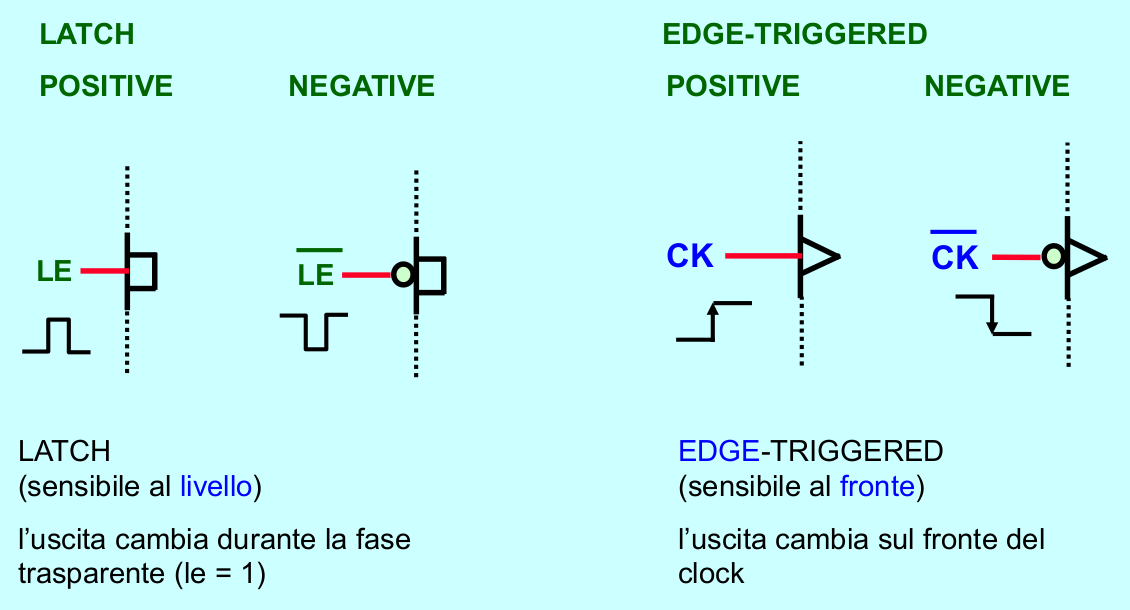
\includegraphics[scale=0.30]{tipi-di-ff.png}
\end{figure}

Il FF-JK ci permette di avere delle funzionalit\`a leggermente pi\`u complesse: con le due entrate a $0$ il valore di $Q$ viene mantenuto lo stato precedente, con $J$ a $1$ $Q$ va a $1$, con $K$ a $1$ $Q$ va a $0$, con $J$ e $K$ entrambi a $1$ l'uscita assume $Q*$ (lo stato al clock predente ma negato).
\begin{figure}[H]
    \centering
    \begin{circuitikz}
        \ctikzset{logic ports/scale=0.7,logic ports/fill=yellow}
        \draw node[flipflop SR] (ff) {};
        \draw (ff.pin 1) -- ++(-0.5, 0) node[and port, anchor=out] (AND1) {}
        (AND1.in 2) to node[left] (term) {J} ++(-0.2, 0);
        \draw (ff.pin 3) -- (ff.pin 3 -| AND1.out) node[and port, anchor=out] (AND2) {}
        (AND2.in 1) to node[left] {K} ++(-0.2, 0);
        \draw (ff.bpin 2) -- (ff.bpin 2 -| term.east) node[left] {CK};
        \draw (ff.pin 4) to[short,-o] ++(1.7, 0)
        (ff.pin 4) ++(1, 0)  node[coordinate] (a) {} to[short,*-] (ff.up -| a.center) -| (AND1.in 1);
        \draw (ff.pin 6) to[short,-o] ++(1.7, 0)
        (ff.pin 6) ++(.7, 0)  node[coordinate] (b) {} to[short,*-] (ff.down -| b.center) -| (AND2.in 2);
    \end{circuitikz}
\end{figure}


\subsection{Ritardi nelle Porte Loiche Sequenziali}
\paragraph{FF-SR}
Le porte NOR introducono dei ritardi, per far si che i cambiamenti abbiano effetto, i comandi di SET e RESET devono avere una durata minima (di solito il doppio della durata massima del tempo di propagazione nelle porte). Nello porte si ha un ritardo di propagaizone da cui il valore di $Q$ deve arrivare a $Q*$ e viceversa. Se l'intervallo \`e troppo lento il valore di $Q$ rimane invariato, mentre nel caso peggiore rimane in posizione meta-stabile, che va evitato.

\paragraph{FF-D}
Ci sono tre vincoli principali:
\begin{itemize}
    \item Tempi di S e R interni appropriati (come sopra);
    \item Margine di tempo  in cui $D$ deve rimanere stabile nell'intorno del fronte di salta del clock, deve rispettare i tempi di set-up $t_{su}$ e di hold $t_h$, se l'entrata non \`e stabile, nel caso peggiore l'uscita oscilla fino al prossimo colpo di clock.
    \item Durata minima del clock, non deve essere pi\`u veloce del tempo di commutazione;
\end{itemize}

Il ritardo dato dalla della meta-stabilit\`a \`e detto \textbf{tempo di risoluzione}, tra tutti i ritardi non \`e conosciuto a priori, infatti \`e preferibile evitarlo.

Cosa accade con pi\`u FF collegati tra di loro (di solito non accade)? \\
Si deve rispettare il tempo set-up, il tempo della transizione allo stato alto  del segnale, al tempo di hold piu il tempo di discesa.

\subsection{Domande di Fine Capitolo}
\begin{enumerate}
    \item \emph{Un latch nella condizione di trasparenza:} \\
        Mantiene lo stato precedente, anche se l’ingresso varia.

    \item \emph{Quante porte NAND a 2 ingressi servono per realizzare un D-FF (master-slave)?} \\
        6: 4 per i FF, 2 per gli inverter.

    \item \emph{Il D-FF Master-Slave ha una condizione di trasparenza?}
        Si, quando il clock \`e a $1$, il master si travo in trasparenza, mentre quando il clock \`e a $1$ lo slave \`e in trasparenza.

    \item \emph{In un D-latch se D=0, EN=0, PRESET=1, CLEAR=0, Q = ?}
        $Q = 1$

    \item \emph{Tracciare Q per un D-FF con D collegato a Q* (per 4 colpi di CK) se Q inizialmente vale 0.}
        \begin{itemize}
            \item[CK=0:] D = 1; Q = 0;
            \item[CK=1:] D = 0; Q = 1;
            \item[CK=2:] D = 1; Q = 0;
            \item[CK=3:] D = 0; Q = 1;
            \item[CK=4:] D = 1; Q = 0;
        \end{itemize}

    \item \emph{Che cosa sono i tempi di setup e di hold?} \\
        Il tempo di setup \`e l'intervallo di tempo mimino prima del fronte di salita del clock in cui il segnale in ingresso deve rimanere stabile, mentre il tempo di hold \`e l'intervallo minimo dopo il fronte di salita in cui l'entrata deve rimanere stabile.

    \item \emph{Descrivere il comportamento di un FF in condizione metastabile.} \\
        Un FF in condizione metastabile ha delle oscillazioni non definite fino a quando un nuovo colpo di clock ristabilizza il sistema, se non si ha un sistema come un MS allora il FF pu\`o rimanre vicino a tale condizione per un tempo indefinito.
\end{enumerate}


\newpage
\section{Circuiti Sequenziali}
Si \`e visto che \`e possibile rappresetare le informazioni in modo parallelo o seriale. Si possono usare i FF per rappresentare i dati su entrbe le codifiche o per passaere da una all'altra.

\textbf{\emph{A parit\`a di frequenza di clock}}:
\begin{itemize}
    \item Connessione Seriale: piu lenta, piu economica, minor consumo, piu usata su distanze lunghe (SATA, Ethernet)
    \item Connessione Parallela: piu veloce, consumo maggiore di potenza, piu usate su distanze corte (all'interno dei circuiti integrati)
\end{itemize}

Nel momento in cui i FF sono colleagati in serie i dati vengono trasportati in modo sequenziale. Il segnale di ingresso viene ritardato di n-volte tante quante sono i FF. Si puo usare per fare dei filtri digitali (visto a teoria dei segnali). Se si prendono le uscite per ogni FF se possono convertire le informazioni seriali in parallele. \`E possibile usare una variante del circuito per realizzare la trasformazione opposta. Nei CI sono implemente delle funzioni che permettono di far uscire l'informazione in modo seriale,

\subsection{Tipoligie di Registri}
\begin{itemize}
    \item \textbf{PIPO} (Parallel Input Parallel Output): \\
        Possiede N bit, un clock o un latch, comandi vari;
    \item \textbf{SISO} (Serial Input Serial Output): \\
        Una cascata di FF-D con clock e RESET in comune. Viene anche detto reistro a scorrimento (Shift-Register);
    \item \textbf{SIPO} (Serial Input Parallel Output): \\
        Come un SISO ma pu\`o convertier un insieme di dati seriali in parallelo;
    \item \textbf{PISO} (Parallel Input Serial Output): \\
        Permette di carciare in parallelo i singoli FF;
\end{itemize}

Si pu\`o creare un circuito che permette di usare le combinzioni dei tipi conessione sia in input che in output.
\begin{figure}[H]
    \centering
    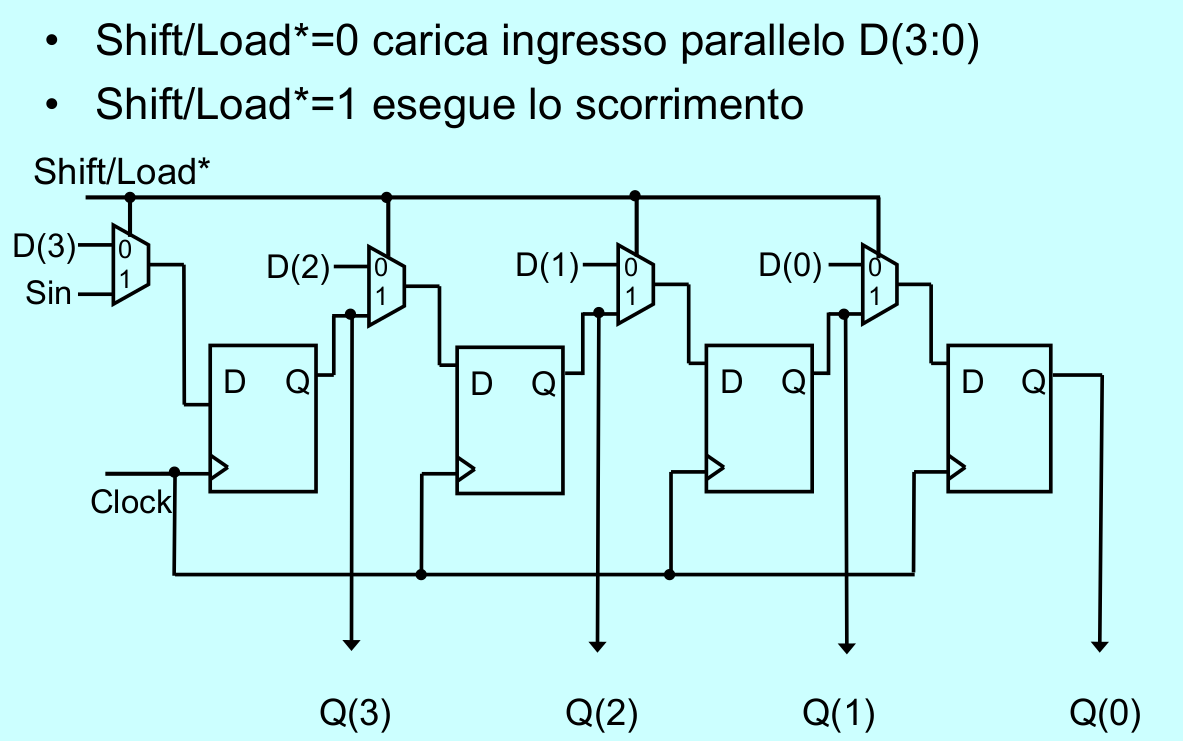
\includegraphics[scale=.3]{shift-register-completo.png}
    \caption{Shift-Register Completo}
    \label{fig:shift-register-completo}
\end{figure}


\begin{example}{Contatore}{contatore}
    Il contatore \`e un contatore in modulo N. Se, per esempio, si vogliono indirizzare le istruzioni, N sar\`a pari al $log_2(\text{numero di indirizzi})$. Il contatore pi\`u semplice da realizzare \`e in modulo 4, si mette l'uscita di un FF all'entrata del clock del prossimo FF, entrambi i FF hanno l'uscita $Q*$ collegata alla propria $D$. Ad ogni colpo di colck $Q1$ e $Q2$ rappresentano il numero del contatore. Il motivo per cui questo \`e un contatore asincorono \`e dato dal fatto che l'entrata CLK del secondo FF non \`e pilota dal clock della CPU ma dall'uscita del primo FF, dunque il ritardo cresce in modo scalare.
    \begin{figure}[H]
        \centering
        \begin{circuitikz}
            \draw node[flipflop D] (ff1) {}
            (ff1.pin 4) to [short,*-] (ff1.pin 4 |- ff1.up) -| (ff1.pin 1);
            \draw (ff1.pin 6) node[coordinate] (pos) {} ++(1.5, 0) node[flipflop D, anchor=pin 1] (ff2) {}
            (ff2.pin 4) to [short,*-] (ff2.pin 4 |- ff2.up) -| (ff2.pin 1)
            (ff1.pin 6) -- (ff2.pin 3);
            \draw (ff2.pin 6) -- ++(0.5, 0);
            \draw (ff1.pin 3) node[left] {CLK} ;
        \end{circuitikz}
        \caption{Contatore in $mod\; 4$}
    \end{figure}
\end{example}

Si possono usare i FF-JK con gli ingressi collegati ad 1 (ad ogni colpo di clock la stato commuta) e CLK negato, si crea cos\`i un contatore che conta oppure no a differenze del segnale in ingresso (contatore con abilitazione).

Si pu\`o realizzare un contatore sicrono usando i FF-JK in combinzione con della logica combinatoria. Le porte AND vanno a verificare quando tutti gli stati precendi sono ad 1, dunque il prossimo stadio commuta e quelli precedenti vanno a 0.

Per realizzare un contatore non in modulo $2^N$ ma, usando un numero qualsiasi si usano le entrate si RESET dei FF. Viene utilizzata una logica combinatoria collegata a tutti i RESET, quando si raggiunge il numero prestabilito tutti i FF vangono porati a 0 e si riparte a contare.

\subsection{Macchina a Stati Finiti}
Per progettare funzionalit\`a pi\`u complicate diventa molto difficile usare solo porte logiche, \`e per questo motivo che viene utilizzato il modello delle \textbf{macchine a stati finiti} (FSM). Le FSM sono fatte da stati iniziali e da stati, ogni stato pu\`o effettuare una transizione ad un altro se sono rispettate delle condizioni. Le uscite verso l'esterno possono essere associate a degli stati o a delle transizioni. Per avere una FSM determinitstica \`e necessario che le condizioni sulle transizioni siano mutuamente esclusive. Le FSM vengono rappresente come dei grafi in cui ogni vertice rappresenta uno stato ed ogni arco rappresenta la condizione di transizione.

In generale c'\`e un interconnessione di porte logiche, che calcolano lo stato futuro a partire dallo stato presente (i valori dei FF) e delle entrate, collegate poi ad un rete combinatoria che produce le uscite. 
Se ci fosse una connessione tra entrate ed uscita la FSM viene detta \textbf{macchina di Mealy}, altrimenti viene detta \textbf{macchina di Moore}.

Si passa da un modello a grafo ad implementazione con porte logiche codificando ogni stato con un simbolo unico, usando ad esempio una codifica binaria. 

\subsection{Analisi dei Ritardi}
Nell'intorno del fronte di salita $(t_r - t_{su}, t_r + t_h)$, si \`e visto come il segnale in ingresso necessita di rimanere stabile. Nel momento in cui viene introdotta una logica si pu\`o analizzare questo ritardo. Ci interessano due ritardi: il minimo ed il massimo, cammino pi\`u corto tra l'uscita di un FF e l'entrata del successivo per tutti i FF del circuito. 

Il massimo \`e correlato alla soddisfazione tempi di setup: ogni volta che c'\`e una trasizione sul clock le uscite dei FF cambieranno, ci sar\`a un ritardo da quando si vede un cambiamento nell'uscita ($t_{}$), ci sar\`a un ritardo causato delle porte logiche ($t_{LCMAX}$). Il periodo di clock non pu\`o essere minore delle somma di questi ritardi.
\[ T_{CLK} > t_{} + t_{LCMAX} + t_{su} \]
Per soddifare il tempo massimo \`e necessario modificare il periodo di clock (molto facile).

Il minimo \`e correlato al tempo di hold (non si deve arrivare al FF successivo troppo velocenmente): le porte logiche hanno bisogno di un tempo minimo per cui ricevano l'uscita delle porte loghiche ($t_{LCMIN}$).
\[ t_h > t_{} + t_{LCMIN} \]
% TODO: chiedere al prof

In generale esistono pi\`u metodi di realizzare la stessa fuznione booleana con dei circuiti combinatori e dei FF. La differenza tra le diverse implementazioni si basa sui ritardi massimi e l'area di silicio occupata, una bouana opprossimazione dell'area occupata \`e data dalla somma dei transistor presenti nel circuitito. 

\begin{example}{}{}
    \emph{Analisi di un circuito sequenziale.} Tracciare il la sequenza di segnali, con stato iniziale $Q_i = 0$ e calcolare la $F_{max}$ del clock, considerando i dati:
    \[ T_{NAND} = 2ns;\quad T_{CKQ} = 3ns;\quad T_{SU} = 1ns;\quad T_H = 1ns;\]
    \begin{figure}[H]
        \centering
        \begin{circuitikz}[scale=0.7, transform shape]
            \draw node[flipflop D,flipflop def={t6=$Q_1$}] (ff1) {FF1}
            (ff1.pin 6) -- ++(2, 0) node[flipflop D,flipflop def={t6=$Q_2$}, anchor=pin 1] (ff2) {FF2};
            \draw (ff1.pin 1) -- ++(-0.5, 0) node[nand port,anchor=out] (nand1) {A};
            \draw (ff1.pin 6) ++(1, 0) node[coordinate] (q1) {}
            (q1.center) to[short,*-] (ff1.up -| q1.center) -- ++(0, 0.2) -| (nand1.in 1);
            \draw (ff2.pin 6) -- (ff2.up -| ff2.pin 6) -- ++(0, 0.7) node[coordinate] (b) {}
            (b.center) -- (b.center -| nand1.in 2) -- ++(-0.4, 0) |- (nand1.in 2);
            \draw (ff1.pin 3) -- ++(0, -1) node[coordinate] (c) {}
            (c.center) -| (ff2.pin 3)
            (c.center) to[short,*-] ++(-1.5, 0) node[left] {CK};
        \end{circuitikz}
    \end{figure}

    Segnali con i rispettivi ritaridi in $ns$.
    \begin{figure}[H]
        \centering
        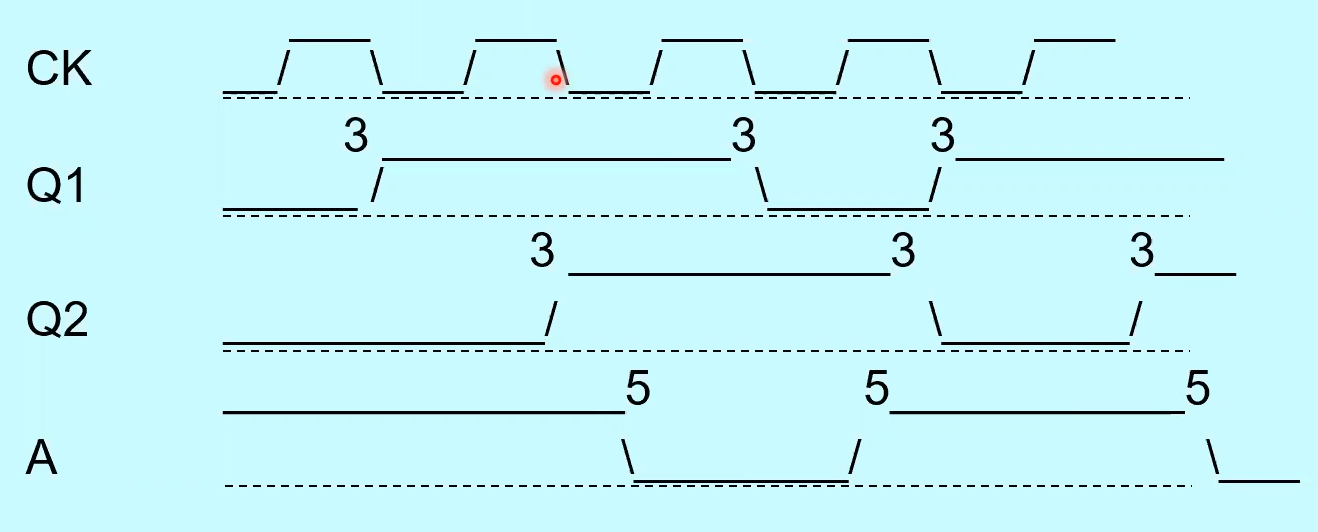
\includegraphics[scale=0.25]{img/segnali-setup-hold-exmp.png}
    \end{figure}


    Il periodo minimo che il clock deve rispettare \`e: $T_{min} > T_{NAND} + T_{CKQ} + T_{SU} = 6ns$
    \[ \to F_{max} = \frac{1}{2ns + 3ns + 1ns} = 166 MHz \]

    Il cammino pi\`u breve da un FF ad un altro va da $Q_2$ a $D_2$, infatti il ritardo minimo della logica combinatoria \`e zero in questo caso. Il vincolo sul tempo di hold \`e rispettato.
    \[ T_H < T_{CKQ} = 2ns \]
\end{example}


\subsection{Domande di Fine Capitolo}
\begin{enumerate}
    \item \emph{Tracciare lo schema di un divisore asincrono modulo 32 realizzato con D-FF.}

    \item \emph{Quanti FF occorrono per realizzare un contatore modulo 17?} \\
        Servon 5 FF.

    \item \emph{Tracciare lo schema logico (porte e FF) di un convertitore da flusso di bit seriale a rappresentazione parallela.} 

    \item \emph{Una FSM ha 9 stati. Quanti FF occorrono per realizzarla?} \\
        Servono 4 FF.

    \item \emph{Si deve realizzare un contatore modulo 4 (FSM controllo della lavatrice). Quale è la massima frequenza operativa se: i FF hanno ritardo di 8 ns; le porte NAND, NOR, NOT e EXOR hanno ritardo di 11 ns; il tempo di setup dei FF è di 9 ns ?} \\
        Per realizzare una AND serve una porta NAND ed una NOT (per il contatore serve una porta XOR ed una AND in serie con una XOR). Il tempo max dello lagica sar\`a $T_{CL} = 11ns\cdot 3 = 33ns$, il tempo minino di clock sar\`a: $T_{CK} = 33ns + 8ns +  9ns = 50ns\quad\to 20MHz$.

    \item \emph{Realizzare un SIPO a 8 bit utilizzando due registri SIPO da 4 bit.} \\
        Si collega il Serial Out del primo al Serial In del secondo.

    \item \emph{Quali parametri determinano la massima frequenza di clock per una FSM?}
        Tempo di ritardo dei FF; massimo tempo di ritardo della logica combinatoria; tempo di setup;
\end{enumerate}


\section{Comparatori}
Un comparatore ha il seguente funzionamento: quando l'ingresso \`e sopra una certa soglia manda l'uscita in H, quando l'ingresso \`e sotto la soglia manda l'uscita in L. Un comparatore viene costrutito usando gli amplificatori operazionali (OP). Per realizzare un comparatore invertente basta invertiere i morsetti. Quando al segnale di entrata viene sommato del rumore si possono creare delle trasiszioni molto veloci, date dal fatto che il segnale oscilla motlte volte attorno alla soglia, il numero alto di transizioni nell'intorno della soglia causano un maggior spreco di potenza. Per risolver questo problema si usano due soglie diverse, una per lo stato da L a H ed una per lo stato da H a L, in questo modo si eliminano le transizioni causate dal rumore, a patto che la soglia del rumore non sia oltrepassata. Un comparatore con queste soglie viene detto \textbf{comparatore con isteresi}, in cui l'intervallo tra le due soglie fa da margine per il rumore.

Il comparatore con isteresi ha due caratteristiche: una quando passa da H a L ed una quando passa da L a H. I comparatori senza isteresi vengono realizzati con OP ad anello aperto, mentre i comparatori con isteresi vengono creati con OP ad anello chiuso con retroazione postiva. 
\begin{figure}[H]
    \centering
    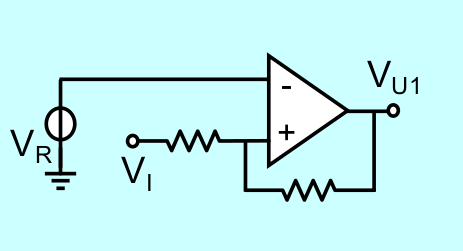
\includegraphics[width=0.4\textwidth]{comparatore-con-insteresi.png}
    \caption{Comparatore con Isteresi}
    \label{fig:comparatore-con-insteresi}
\end{figure}

Nella pratica si compra direttamente il CI con il comparatore e le resistenze che servono a noi. Un comparatore con isteresi \`e anche detto \textbf{Trigger di Schmitt}. Il valori dei threshold dipendono dall'alimentazione e da altri fattori, come tolleranze di fabbricaione.

Utitilizzando i comparatori con isteresi si possono realizzare delle forme d'onda quadra, ci\`o \`e possibile avendo un circuito RC pilotato ad onde quadre, dove la tensione in uscita al condesatore sar\`a una serie di onde, date dalla carica e dalla scarica. Il condensatore messo in retroazione con un comparatore di Shmitt da proprio questo effetto, infatti quando viene oltrepassata la soglia del comparatore il segnale in retroazione sar\`a invertito e dunque porter\`a il condensatore a scaricarsi provocando un'altra transizione della soglia.
\begin{figure}[H]
    \centering
    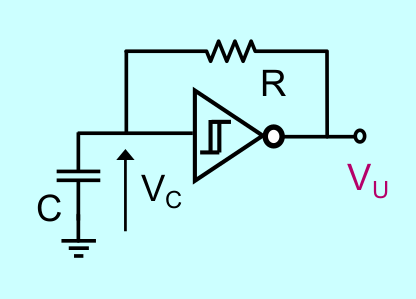
\includegraphics[width=0.35\textwidth]{generatore-onda-quadra.png}
    \caption{Generatore ad Onda Quadra}
    \label{fig:generatore-onda-quadra}
\end{figure}


\subsection{Limiti Operativi}
\textbf{Resistenza di reazione}:
\begin{itemize}
    \item Max: in R deve circolare una corrente maggiore della corrente di ingresso del comparatore;
    \item Min: R \`e vista come carico all'uscita, dunque valori troppo bassi limitano la dinamica di uscita;
\end{itemize}

Il \textbf{condensatore} non ha limiti su quanto pu\`o essere grande, mentre il valore pi\`u piccolo \`e dato dalle capcit\`a parassita di ingresso.

La \textbf{frequenza} minima \`e determinata dalla capacit\`a massima e dalla resistenza massima ($C _{max}, R _{max}$), mentre la frequenza massima \`e determinata dallo slew rate del comparatore.

\subsection{Oscillatori ad Anello}
Un circuito che contiene un numero dispari di inverter diventa un oscillatore, il circuito diventa instabile, dove il periodo dell'oscillazione \`e dato dalla somma delle propagazioni in salita ed in discesa degli inverter, tante volte quante sono gli inverter. Si usano gli inverter per creare degli oscillatori perch\`e le resistenza e le capacit\`a fisse dei circuiti con i comparatori sono pi\`u costose e pi\`u imprecise.

Per riuscire a migliore la precisione delgi inverter bisongna inserire nella rete di reazione un oggetto che migliora la precisione.

Si utilizza il quarzo (materiale piezoelettrico), che risponde ad una tensione con delle oscillazioni molto precise, ha come modello elttrico una combinazione accordata di resistenze e capacit\`a. L'utilizzo di cristalli al quarzo \`e il metodo pi\`u economico per realizzare degli oscillatori. La resistenza di reazione serve per permettere al quarzo di operare in condizioni favorevoli.


Per controllare la frequenza di clock bisongna essere precisi ma flessibili: nel caso in cui il carico computazionale varii nel tempo (eg sistema di un celluare, dove il carico viene ragolato a differenza delle operazioni che devono eseguire). In questo caso si usanao gli \textbf{anelli ad aggancio di fase} (PLL: Phase-Locked Loop). Usando le reazione per controllare la frequnza, un oscillatore controllato in tensione pu\`o anche non essere preciso, questa imprecisione verr\`a attenuata proprio dalla rezione.
\begin{figure}[H]
    \centering
    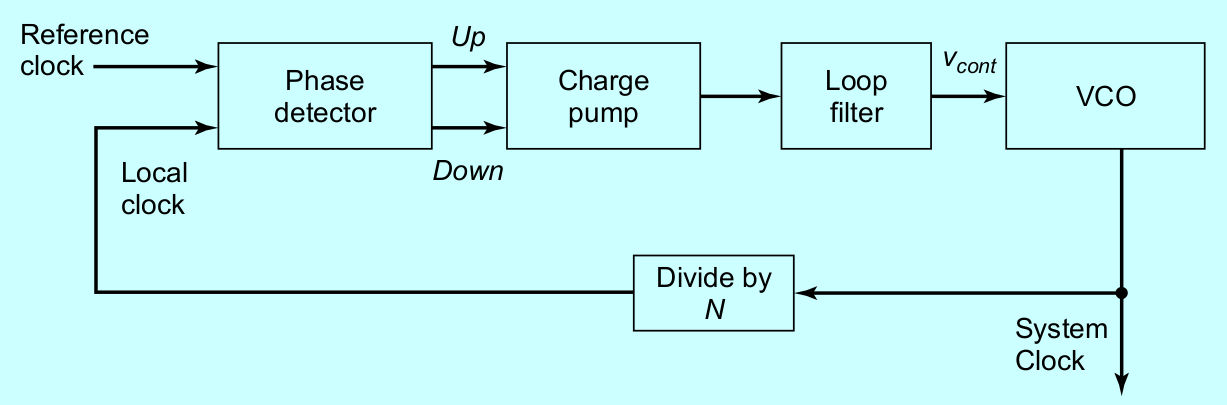
\includegraphics[width=0.8\textwidth]{pll.png}
    \caption{Phase-Locked Loop}
    \label{fig:pll}
\end{figure}

\begin{itemize}
    \item \textbf{Rivelatore di fase:} indica se la frequnza deve salire o scendere. Cicruito logico che verifica quale dei due segnali arriva prima, aumenta o diminuisce in reazione la frequenza dell'oscillatore, mantenendo allineate le due fasi.
    \item \textbf{Charge Pump:} transforma il comando ''vai su'' o ''vai giu'' del rilavatore di fase in tesioni, regolondo le tesione di alimentazione della catena degli inverter in modo continuo.
    \item \textbf{VCO (Voltage-Controlled Oscillator:} Il charge pump da piccoli impulsi in modo da aumentare o diminuire la tensione di alimentazione, infatti un inverter ha una frequenza minore al diminuire della tensione di alimentazine e vicerversa.  L'anello di reazione aggancia il VCO all'oscillatore di riferimento, con alta precisione e con una frequenza minore. La tesione di uscita andr\`a poi andra ai FF del circuito.
\end{itemize}

Per ridurre la potenza si puo ridurre la tensione di alimentazione del circuito o si pu\`o abbassare la frequenza.


\subsection{Domande di Fine Capitolo}
\begin{enumerate}
    \item \emph{Quali parametri descrivono un comparatore di soglia?} \\
        Se ha isterisi oppure no, valori della tensione di uscita e valori delle tensioni di soglia

    \item \emph{Per quale motivo i comparatori hanno isteresi ?} \\
        Per ridurre l'influenza del rumore. Causa molte commutazioni in uscita con maggiore spreco di potenza.

    \item \emph{Tracciare lo schema di un generatore di onda quadra, e indicare cosa determina le frequenze massima e minima ottenibili} \\
        Schema in (\autoref{fig:generatore-onda-quadra}). La frequenza minima \`e determinata dai valori massimi di resistenza e capacita, mentre quella massima da quanta corrente si \`e in grado di alimentare la capacit\`a e da quanto grande 'e la capacit\`a (slew rate).

    \item \emph{In un generatore di onda quadra con integratore e trigger, come cambia la frequenza raddoppiando la capacità dell’integratore?} \\
        La frequenza raddoopia.

    \item \emph{Perché non si usano gli oscillatori ad anello per generare un clock stabile?} \\
        Perche i parametri di questi oscillatori cambiano con la temperatura, \`e difficile travare errori bassi nelle capacit\`a e nelle resistenza. Non si puo vendere un componente con un incertezza dell $1\%$ sulla frequenza.

    \item \emph{Quali sono i vantaggi degli oscillatori a quarzo?} \\
        Gli oscillatori al quarzo sono molto precisi, possono oscillare a frequenze molto alte, sono molto precisi, sono molto economici da realizzare.

    \item \emph{Perché si usa un PLL per generare frequenze di clock dell’ordine dei GHz?} \\
        Usando i PLL si puo ridurre la frequenza quando non \`e necessario, creare un oscillatore al quarzo che gira sui GHz \`e molto costoso, inoltre la precisione deve essre molto alta.
\end{enumerate}



\newpage
\section{Logiche Programmabili}
I primi CI sono usciti negli anni '60, creati interamente sul silicio con BJT. Nel '71 si passa ad usare i MOS, con un consumo di postenza molto minore $ \implies $ aumento del numero di transistor sul CI. La \textbf{Legge di Moore} \`e una legge economica che stabilisce una relazione econuumica tra i produttori dei CI ed i consumatori, la legge di Moore dice che: il numero di trasistor raddoppia sulla superficie del silicio ogni 2 anni. Questo \`e possibile perch\`e la dimensione dei transistor si riduce, ma intorno al 2010, arrivati intorno ai $30nm$ di lunghezza di un singolo transistor, la velocit\`a \`e dimuita. Per drogare il canale vengono usati pochi atomi, addirittura 2-3, dunque le differernze tra transistor possono addirittura variare del $50\%$ o $30\%$. Per questo motivo si \`e aumento il numero di core, con un conseguente aumento della quantita di silicio, con un aumento dei prezzi. Il motivo per cui il costo dei trasistor cresce \`e dato al fatto che: le maschere per creare il CI diventano sempre pi\`u costose, per generare, i CI servono sempre pi\`u maschere attroverso l'uso dell'interferenza dei raggi.

Il costo di un CI \`e dato da: il costo delle maschere ed il costo di progettazione che \`e un costo \emph{una tantum} (NRE cost: Non-Recurring Engineer cost), che diviso per il numero di CI si somma al costo unitario di produzione.

Ci sono essenzialmente 4 tipi di CI:
\begin{itemize}
    \item Comodity (Commercial Off The Shlef): processori, memorie, (usati in ampiamente, con costi solo per il silicio);
    \item Custom: circuiti specializzati (come circuititi di potenza, analogici, ...);
    \item Semicustom: ad esempio la Apple che vende il suo prodotto con il suo HW, ha bisogno di un gruppo che progetta un codice che giri su l'HW ed un gruppo che progetti l'HW, si hanno elevati costi di progettazione, ma il prodotto \`e molto performante;
    \item Circuiti Logici Programmabili: ci sta un codice che pilota i transistor, potendo cambiare il funzionamento delle porte logiche a piacimento.
\end{itemize}

Quando un'azienda non pu\`o permettersi di svilupppare internamente un prodotto compra un'azienda che lo puo costruire, o ne compra i diritti di utilizzo. Comprare componenti o un'azienda intera \`e necessario all'interno dell'industria elettronica, dato degli enormi costi dello sviluppo, ci\`o permette di creare sistemi molto complessi. Il problema risiede nel mettere insieme tutto ci\`o, per capirne le specifice e determinare come tutti questi componenti vanno ad integrarsi tra di loro.

La segmentazione dell'industria \`e la seguente:
\begin{itemize}
    \item \textbf{Progetto di sistemi:} (Marelli) miglia di aziende fanno progetti di sistemi, grandi o piccoli. A volte pu\`o includere la produzione;
    \item \textbf{Progetto di circuititi integrati:} (Apple, ARM) aziende specializzate per gli alti costi degli NRE e delle maschere;
    \item \textbf{Fabbricazione di circuiti integrati:} (Intel, Samsung) molto specializzata per gli altissimi costi degli impianti di produzione.
\end{itemize}

Nel caso dei circuti full custom si lavora a tutti i passi del progetto manualmente. Si ha la totale flessibilit\`a ma i costi sono altissimi, si puo fare solo per circuititi con circa 200 transistor, le memorie sono dei circuititi full custum;

Circuiti Semicustum: sono progettati a partire da porte logiche, chi progetta questi circuti ha a disposizione una libreria di porte che si possono utilizzare nel circuito, non si \`e necessario calcolare le posizioni all'interno del silicio.

Circuiti Programmabili: si decide tramite software come le porte si dovranno comportare. I CI Programmabili sono a met\`a tra spese e tempi di produzione. 

\subsection{Componenti Programmabili}
L'asppetto fondamentalo \`e l'elevato numero di clienti per tali circuiti, dunque il prezzo di progetto viene spalmato sulle grandi quantit\`a vendute. Il CI deve essere molto flessibile per includere una grande quantit\`a di casi. I CI possono essere programmati permanentemente o riprogrammabili dinamicamente (tipicamente si usa in fase di prototipazione). Un esempio di CI riprogrammabile on the fly, sono le base station delle reti cellulari che hanno visto upgrade di protocolli e di getsione dei dati.

La configurazione \`e memorizzata in memoria. Un CI programmabile \`e fatto da:
\begin{itemize}
    \item Memoria
    \item Fuznione logiche relizzate con tabelle di lookup o 
\end{itemize}

Programmabel Logic Array (PLA): fatte da matrici di invertitori porte AND e OR. I fili vengono bruciati per creare i ponti di collegamento che andranno a creare le funzioni logiche.
\begin{figure}[H]
    \centering
    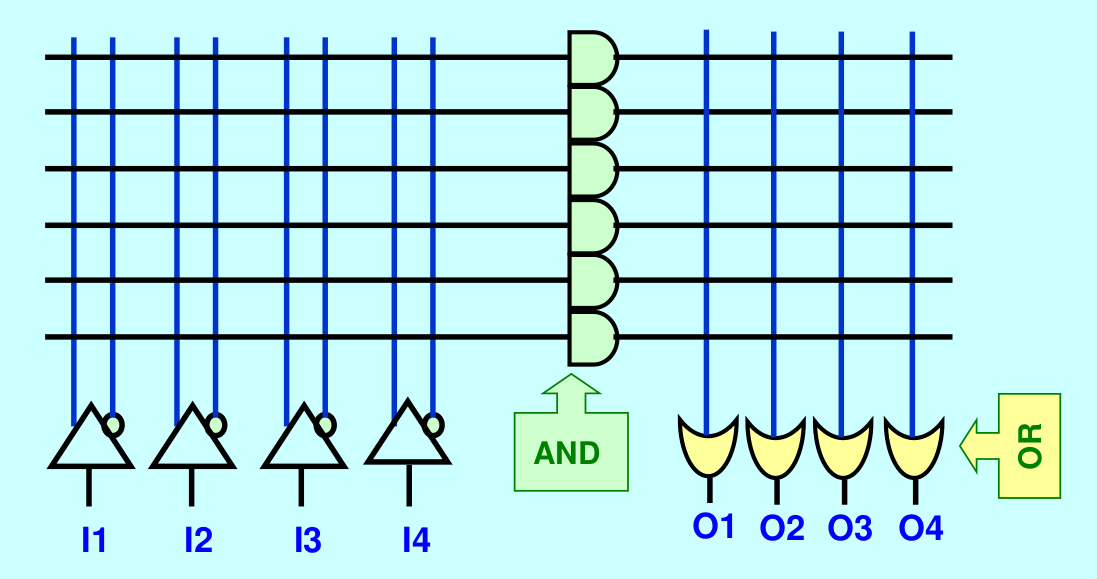
\includegraphics[width=0.55\textwidth]{pla-logic.png}
    \caption{Logiaca PLA}
    \label{fig:pla-logig}
\end{figure}

Field Programmabel Gate Array (FPGA): fatta da celle logiche che realizzano qualsiasi funzione logica fino ad un certo numero di ingressi in cui sono presenti anche dei registri. Le connessioni sono anche programmabili e le celle di ingresso ed uscita consentono di collegare il circuito con un circuito stampato. Ogni cella ha una memoria in cui si mette le fuzione logica, si possono realizzare quasi tutte le combinazioni di fuznioni con un N ingressi. La memoria pu\`o esser caricata su una RAM, dei registri (volatile), o memorie non volatili in cui si usano fusibili, queste ultime si usa perch\`e sono immuni al fenomeno di distruzione causto dai raggi cosmici.

% TODO:  <26-03-22, finire> %

\subsection{Domande di Fine Capitolo}
\begin{enumerate}
    \item \emph{Descrivere da cosa dipende il costo di un circuito integrato.} \\
        Dal costo di produzione e dal costo di progettazione.

    \item \emph{Perché il progetto deve essere rapido?} \\
        Perch\`e se il progetto viene distribuito troppo tardi la finestra di mercato ha un tempo finito, dunque il coomponente fatturer\`a fintanto che la finestra rimane aperta. Con un distribuizione ritardata il prezzo dei costi di produzione non si riesce a colmare.

    \item \emph{Cosa significa “COTS”?} \\
        Vuol dire Commercial Off-The-Shelf. Sono dei componenti dedicati al general purpose.

    \item \emph{Spiegare le differenze tra full custom, semicustom, logiche programmabili.} \\
        Le full custom sono circuiti progettati al livello delle porte logiche, hanno alti costi progettuali. Le semicustom usano moduli gi\`a utilizzati ed assemblati instieme, con costi di produzione medi. Le logiche programmabili

    \item \emph{Quali sono i vantaggi delle logiche programmabili?} \\
        Quando si hanno pruduzioni relativamente piccole ma non si vuole un CI che consumi troppo, sono intermedi sia in termini di effecenza che in termini di programmazione.

    \item \emph{Per quali applicazioni un componente logico programmabile è più indicato di un microprocessore?} \\
        Applicazione ad elevate prestazione e con un elevato numero di componenti venduti.

    \item \emph{Elencare le tecnologie di memoria usabili nei circuiti logici programmabili.} \\
        RAM; Registri; PROM; EPROM; EEPROM; FLASH.

    \item \emph{Quando è conveniente realizzare sistemi elettronici su componenti programmabili?} \\
        --
\end{enumerate}




\newpage
\section{Verilog}
Il Verilog \`e un linguaggio di programmazione con la concorrenza come aspetto principale, descrivendo il comportamento dei vari moduli. Esistono anche altri linguaggi come il VHDL e SystemC. L'idea per la nascita di verilog \`e simulare il comportamento di un circuito logico.

La sintassi del Varilog \`e molto simile al C. Un modulo \`e un componente elettronico che pu\`o essere usato con degli ingressi e delle uscite:
\begin{itemize}
    \item Definizione del modulo: le uscite vanno prima degli ingressi;
    \item Lista di porte;
    \item Lista delle dichiarazioni delle porte;
    \item Dichiarazione dei parametri;
    \item Istruzioni del preprocessore;
    \item Descrizione del comportamento tra un modulo;
\end{itemize}

Il modello di programmazione base nel varilog sono le porte logiche primitive. Ogni segale interno al modulo va definito come \texttt{wire}, le porte sono definite implicitamente come \texttt{wire}.

Per descrivere i ritardi si una il \texttt{\#}. Un ritardo ha la forma:
\[ \texttt{\#(Tp);}\quad \texttt{\#(Tmin:Typ:Tmax);}\quad \texttt{\#(Tplh, Tphl);} \]

L'unit\`a di misure \`e definita da una direttiva:
\begin{lstlisting}[language=verilog]
    `timescale <time_unit>/<time_precision>
\end{lstlisting}

\begin{example}{Half Adder Modulo}{half-adder-modulo}
\begin{lstlisting}[language=verilog]
module hadd(Sum, Carry, X, Y);
input X, Y;
output Sum, Carry;

xor #(2:3:4, 5) (Sum, X, Y);
and #(3.567) (Carry, X, Y);
endmodule
\end{lstlisting}
\end{example}

Si possono creare pi\`u istanza di un modulo anche dando un nome. 
\begin{lstlisting}[language=verilog]
    ...
    hadd M1 (...)
    hadd M2 (...)
\end{lstlisting}

Le assegnazioni continue sono uno dei modi di assegnazione dai registri. \`E un modo ad alto livello di assegnazione della logica combinatoria, dove il tempo \`e scandito dal segnale di clock e le assegnazioni avvengono quando un operando cambia valore. Le espressioni possono contenere espressioni booleane aritmetiche. La destinazione deve essere \texttt{wire}:
\begin{lstlisting}[language=verilog]
assign out = a & b | c;   // espressione booleana
assign eq = (a + b == c); // soommatore e comparatore
wire #10 inv = ~in;       // inverter con ritardo 10 time unit
wire [7:0] c = a + b;     // somma a 8 bit
\end{lstlisting}

\begin{example}{Porta myXOR}{porta-myxor}
\begin{lstlisting}[language=verilog]
module my_xor(C,A,B)
output C;
intput A, B;

assign #2 C = (A ^ B);
endmodule
\end{lstlisting}
    2 timeunit dopo che A o B sono cambiati di valore il risulatato di A xor B viene assegnato a C.

    IMPORTANTE: I ritardi servono solo per simulazione, \underline{non hanno significato} per la sintesi.
\end{example}


\begin{example}{Sommatore a 4 bit}{sommatore-a-4-bit}
\begin{lstlisting}[language=verilog]
module adder4 (Sum, Cout, A, B, Cin);
input [3:0] A, B;
input Cin;
output [3:0] Sum;
output Cout;
assign {Cout, Sum} = A + B + Cin;
endmodule
\end{lstlisting}
    \{Cout, S\} \`e un concatenazione di bit.
\end{example}

Si possono usare variabili definite con la keyword \texttt{parameter}, che sono ridefinibili durante l'instanziazione del modulo.

Quando si usa un modulo si possono usare le nominazioni dei parametri e delgi argomenti, questo \`e utile quando si hanno centinaia di argomenti e parametri.
\begin{lstlisting}[language=verilog]
adder adder_8 #(8) (co, s, a, b, ci);
adder adder_8 #(width=8) (.a(a), .b(b),
    .cin(ci), .cout(co), .sum(su));
\end{lstlisting}

Si possono lasciare dell uscite non connesse non nominando gli argomenti durante l'instaziazione.

Gli \textbf{always block} sono processi concorrenti, rappresentati come blocchi di codice procedurale che contengono istruzioni sequenziali in cui l'ordine di moduli ed instaziazione non conta. L'always posside una \textbf{sensitivity list} che definisce esattamente quando un always block viene eseguito una volta dalla prima istruzione all'ultime. Un'always pu\`o essere:
\begin{itemize}
    \item attivo sul livello (latch o logica combinatoria):
\begin{lstlisting}[language=verilog]
always @(a or b) || always @(*) 
                            \|
    tutti i segnali che compaino sulle espressioni
\end{lstlisting}

    \item attivo sul fronte (FF sincrono):
\begin{lstlisting}[language=verilog]
always @(posedge Clock or Reset) 
\end{lstlisting}
\end{itemize}

In verilog esistono due tipi di dato, quelli senza memoria \texttt{wire} e quelli con memoria \texttt{reg}. I \texttt{wire} sono le usciute di tutti gli \texttt{assignment}, i \texttt{reg} sono le uscite di tutti gli always block.

Esistono anche delle espressioni condizionali con cui si possono creare ad esempio le istruzioni di una ALU:
\begin{lstlisting}[language=verilog]
if( alu_func == 2`b00)
    aluout = a + b;
else if( alu_func == 2`b01)
    aluout = a - b;
else if( alu_func == 2`b10)
    aluout = a & b;
else
    aluout = a | b;
end
\end{lstlisting}

Usando gli switch-case si possono usare dei don't care per effettuare delle minimizzazioni.

Per modellare un latch si usa un modo canonico che tutti i sintetizzatori possono capire.
\begin{lstlisting}[language=verilog]
module latch (CLK, Reset, D, Q);
input CLK, Reset;
input D;
output reg Q;

always @(D or Reset or CLK) begin
    if(Reset)
        Q = 0;
    else if(CLK)
        Q = D;
end;
endmodule
\end{lstlisting}

0ppure un FF con reset sincrono:
\begin{lstlisting}[language=verilog]
module FF (CLK, Reset, D, Q);
input CLK, Reset;
output D;
output reg Q;

always @(posedge CLK) begin
    if(Reset)
        Q = 0;
    else if(CLK)
        Q = D;
end;
endmodule
\end{lstlisting}


\subsection{Flusso di Progetto}
Passa attraverso dei passi standard. 
\begin{enumerate}
    \item L'ingresso \`e il modello RTL della funzionalit\`a da relizzare;
    \item Verifica delle specifiche, con la simulazione a livello funzionale, all'ingresso della simulazione si possono introdurre delle test bench scritte in verilog;
    \item Si effettua la sintesi logica, ad esempio: periodo di clock che si vuole utilizzare, ecc... ottenendo un circuito logico che corrisponde alla funzionalit\`a di quello in entrata;
    \item Il circuito creato dalla sintesi logica verr\`a piazzato sulla FPGA, decidnendo lo posizione fisica dei blocchi e le modalit\`a di collegamento;
    \item Viene genereato un bit-stream: volori che verrano caricati dentro l'FPGA per configuralrla.
\end{enumerate}

Sintesi Logica: \\
Fa un lavoro di compilazione, crearo attraverso la semntica del linguaggio, un circuito corrispondente non ottimizzato. Si usano in una fase successiva, i teoremi dell'algebra booleana per minimizzare il numero di porte logiche, minimizzando costi e ritardi. L'uscita della sintesi logica sono un insieme di porte collegate tra di loro, scritte in un liguaggio per descrivere i circuti. Si ottiene anche un'approssimazione dei tempi di ritardo (si sapranno solo quando i circuiti saranno piazzati sul silicio). Usata l'algebra booleana si traducono gli insiemi di porte in look up table (LUT). Una volta ottenute le LUT si possono andare a piazzare sul silicio, cercando di minimizzare la lunghezza delle interconnessioni.

--

Per progrettare gli ASIC, si spende un tempo motlo maggiore per verifcare che nel circuito non siano presenti dei bug. Le verifiche costano molto di pi\`u.

Flusso per ASIC
\begin{enumerate}
    \item Verifica del codice verilog;

        --

    \item Test Insertion: si inserice della logica per collaudare il circuito;
    \item Analisi dei ritardi;
    \item Fase dei piazzamento delle interconnessioni;
    \item Tracciamento dell'albero del clock (molto difficile);
    \item Fase di estrazione delle maschere fisiche, si effettua la verifica che la logica della maschere sia effettivamente uguale alla logica RTL.
\end{enumerate}

In FPGA le porte sono gi\`a piazzate sul silicio, in cui le LUT vanno piazzate, mentre negli ASIC l'organizzazione \`e piazzata su delle righe (simil pali della luce), un cattivo piazzamento pu\`o causare delle lunghe interconnessione che cuasa delle congestioni (frequenza minore).

Dopo la fase di piazzamento vengono effettuate le interconnessioni. Si usano algoritmi come quello di Dijkstra, tenendo conto dei ritradi e delle congestioni.


\newpage
\section{Memorie a Semiconduttore}
Classificaionzi:
\begin{itemize}
    \item Possono essere sia lette che scritte;
    \item Possono essere 
\end{itemize}

Tutte le memorie usano dei protocolli di accesso, che vengono attuati attraverso dei segnali di controllo (molto simili al clock), i dati possono essere letti o scritti dopo un tempo di stabilizzazione. In questo caso possiamo avere due tipi di segnali: READ e WRITE. Il motivo per cui i segnali sono separate \`e perch\'e i dati letti e scritti viaggiano sugli stessi circuiti. Ci sono dei ritrdi minimi e massini tra le letture e le scritture. Nei FF questi ritardi sono unici, nelle memorie i tempi minimi sono molto differenti.

Da un punto di vista logica le memoria sono organizzate in gruppi di parole in cui ogni parola ha un'indirizzo, ogni lettura trascferisce una quantit\`a di dati in blocchi di parole. Internamente l'architettura \`e organizzata in una matrice approssivativamente quadra, minimizzando le lunghezze, di fatto l'indirizzo a N bit viene suddiviso in due parti, una che seleziona la riga ed una che seleziona la colonna.

Le righe attivano la \textbf{wordline}.

\subsection{DRAM}
Tra le memorie la DRAM ha la cella di memoria pi\`u piccola, formata da:
\begin{itemize}
    \item Un filo di bitline;
    \item Un filo di wordline;
    \item Un transistorn permette di caricare la capacit\`a $C_S$, questa ccapacit\`a perde continuamente elettroni duvuto alla corrente di perdita del trasistor, se il potenziale \`e basso si legge L se il potenziale \`e alto si legge H, questa capcit\`a \`e molto piccola (perch\`e si vuole usare la minor area), \`e pi\`u piccola delle capacit\`a parassite del filo di BL. In scrittura si attiva la wordline e si porta la capacit\`a a potenziale alto o basso. In lettura BL viene caricata $V_{dd}/2$, \`e pi\`u facile caricare o scaricare di poco la line, il valore reale sar\`a eleborato successivamente con dei circuiti differenziali.
\end{itemize}

% TODO:  <29-03-22, controllare reg per battuta sul cappio, minuto 30 in  poi> %

Fatta una lettura il dato viene distrutto, quindi dopo ogni lettura una riga deve essere riscritta, in questo modo viene anche ripristinato dalle correnti di perdita. Queste operazioni di riscrittura devo essere fatte periodicamente, questa operazione viene nominata \textbf{rinfresco}, in memorie questa procedura viene implementata automaticamente a livello di HW.

Per la lettura viene usata una cella di memoria caricata a $V _{dd}/2$, il seganle letto e il segnale della cella dummy viene mandato in un amplificatore differenziale. Questo viene fatto per minimizzare il disturbo dal rumore, essendo le due wordline in parallelo hanno gli stessi disturbi (eliminati dall'amplificatore differenziale).

...

L'operazione di pilotaggio dei Sense Amplifier sono molto pi\`u lente delle logica combinatoria. 

...

Avere tante sotto RAM piccoline migliora la velocit\`a, diminuendo le capacit\`a parassita del BL.

...

Uno dei primi metodi di lettura \`a la \textbf{fast page page mode} (o \textbf{burst}), in cui si leggono le colonnes successive alla parola letta, molto veloce.

Oggi le RAM sono tutte sincrone (hanno un clock che temporizza), inoltre 

...

Si possono usare le pipeline con una \textbf{burst lenght}, mentre si legge una riga si preparano le parole successive. I burst possono essere usati sia in lettura che in scrittura.


\subsection{SRAM}
Si possono usare gli inverter per realizzare. Ci servono due BL complementate, il motivo \`e che non risuciremmo a invertire lo stato del circuito bistabile. La velocit\`a \`e dell'ordine della logica combinatoria. Ci sono dei trasistor di precarica che portano ...

Il sense amplifier \`e fatto da un

Come la DRAM abbiamo il WE ed il OE (Write Enable e Output Enable). Oggi si usano le SRAM sincrone 

All'interno della RAM sono presenti delle parti di memoria ridontdai per correggere gli errori. Per momorizzare i bit si usano dei codi di autocorrezione, oppure segnalare un errore. Al posto di usare memoria sul silicio ridondante si possono usare questi codici di autocorrezione. 

\subsection{Memorie Indirizzabili a Contenuto} (CAM) (Content Addressable Memory)
Al contrario delle RAM diciamo il contenuto che ci interessa e risponde con l'indirizzo o gli indirizzi a cui i volori corrispondono (potreebbe anche non esistere).

Il ciclo di scrittura funziona alla stesso modo delle RAM. 

Per leggere l'indirizzo si utilizza un modo molto simile all'indirizzamento dei pacchetti IP. La CAM viene usata ad esmepio nelle cache.

\subsection{Memorie Non-Volatili}
Queste memorie possono essere di tue tipi differenti:
\begin{itemize}
    \item Read-Only: la memoria pu\`o essere scritta solo in fase di programmazione
    \item Riprogrammabili: possono essere riscrivibili, questo per\`o prende pi\`u tempo
\end{itemize}

Nelle RO si usano i transistor per portare a livillo basso o alto il segnale, mettre si usa un circutito vuoto per il complementare.

Si usano i transistor come pull-up perch\'e sarebbe pi\`u complicata fare una resistenza su un transistor.

Anche se oggi non sono pi\`u usate i due tipi di NAND e NOR vengono ancora usato nelle memorie riprogrammabili.


% TODO:  <29-03-22, finire> %

\subsection{FLASH}
% TODO: finire %
Le momerie flash (vengono dette cosi perch\`e quando viene effettuata la scrittura \`e fatta a blocchi di parole). Per creare i bit si iniettano delle carica nei gate flottanti. (NOR) Per cancellare la carica iniettiamo una carica negativa sul gate flottante, che andra\`a a schermare il pontenziale positivo della WL evitando che si formi il canale sulla BL.

(NAND) Si iniettano cariche positive sul gate flottante molto.
SSL e GSL selezionano alcuni blocchi all'interno della Flash.

NAND Flash:
si fa tunneling per iniettare le cariche nel canale, per mandare via le cariche si usa usa un potenziale alto sul canale.
La struttura predominante \`e quella orizzontale. Per sfruttare pi\`u spazio su usa la terza dimensione.

Le flash sfruttano a pieno la terza dimensione.

Le scritture singole sono possibili solo sulle NOR, mentre la riscrittura a blocchi \`e possibile su entrambe. La lettura a accesso casule della NAND \`e 200 volte pi\`u lenta della NOR, per il primo accesso, mentre la lettura delle parole adiacenti \`e molto veloce.
Le operazioni di scrittura sono pi\`u veloci nella NAND, la banda di scrittura \`e molto maggiore nelle NAND.
Eliminare un blocco nella NOR \`e molto pi\`u lento che nelle NAND perch\`e si deve cancellare la carica dei singoli transistor.

Le operazione sulla FLASH:
La scrittura individuale si pu\`o fare solo settndo a 0. Dunque si deve prima mettere tutto il blocco ad 1 e poi andare a mettere gli zeri ad ogni cella.

L'organizzazione \`e suddiva in: blocchi, pagine, byte. (La cancellazione avviene suli blocchi).

La vita di una memoria riprogrammabile \`e finita, gli elettroni passano attraverso ed ad ogni riprogrammazione il materiale si rovina, dunque dopo un numero di cicli di scrittura i gate non pi\`u a mantenere le cariche. Allora hanno bisgno di un controllore delle memoria intelligente che distribuisce le momoria uniformemente nei vari blocchi, in modo da evitare la rottura.



\newpage
\section{Interconnessioni}
I problemi dei sistemi di interconnessione sono divisi per: potenza (trasporto di energia), segnali (trasporto dell'informazione). La priorit\`a nelle linee di interconnessione \`e l'\textbf{integrit\`a del segnale}: mantenere l'informazione consistente. Le linee di interconnessione per trasferire dei dati usano un livello basso ed uno alto, interpretati come zeri e uni che sono valori interpretati da tensioni e correnti.

\subsection{Rumore Temporale}
Supponiamo di avere due segnali che hanno delle transizioni, questi due segnali rappresentano i dati da trasferire e devono essere sincroni, pu\`o accadere che le transizioni non siano sincrone tra di loro, la differenza temporale tra le transizioni dei segnali \`e detta \textbf{skew} $t_K$. Supponiamo invece di avere un segnale che possiede una temporizzazione (ovvere deve avere una transizione in un dato momento), ma questa avviene in anticipo o in ritardo, il tempo di ritardo \`e detto \textbf{jitter} $t_J$. Jitter e Skew portano a problemi di temporizzazione dei segnali.

Un modello ideale di interconnessione \`e un filo equipotenziale senza rumori tra il driver ed il receiver. In generale per analizzare il passaggio delle informazioni si usa un modello ISO/OSI, quindi vengono usate delle interfaccie che comunicano con gli stessi livelli. Si studiano i livelli pi\`u bassi: livello fisico e data link. 

\subsection{Livello Elettrico}
Le linee di interconnessione che si trovano a livello fisico (correnti e tensioni), collegano dei circuiti digitali da dei driver e da dei reciver che convertono il segnale da digitale ad analogico e viceversa. Gli obbiettivi sono: la massima velocit\`a ed assenza di errori. 

Un driver viene modellato come un generatore di tensione in serie con un resistenza, mentre un reciver \`e modellato come con resistenza a massa (di solito infinita) ed una capacit\`a a massa, che comporta un ritardo nelle transizioni.
\begin{figure}[H]
    \centering
    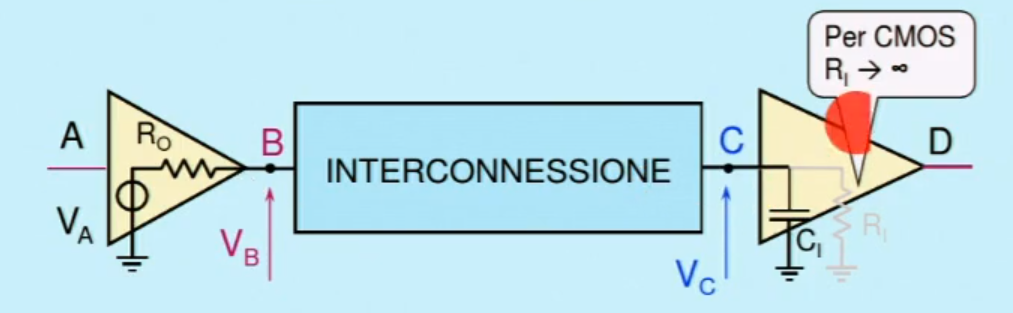
\includegraphics[width=0.5\textwidth]{modello_driver_reciver.png}
    \caption{Modello Driver Reciver}
    \label{fig:modello_driver_reciver}
\end{figure}

Per modellare un linea di interconnessione si possono usare diversi approcci. Un modello ideale \`e una linea equipotenziale. Un modello pi\`u relistico \`e un modello RC, in cui i tempi di ritardo dipendo dalla costante di tempo $\tau = RC$ e dalla tensione di soglia, il ritardo massimo dipende da $V _{IH}$ mentre il tempo minimo dipende da $V _{IL}$.

Il ritardo con cui viene rilevata una rilevata una variazione di stato logico \`e detto ritardo di trasmissione (anche detto ritrado di propagazione nel modello simplificato) $t _{TX}$. Quando si ha una variazione della costante di tempo si hanno due tempi di ritardo, uno minimo ed uno massimo: per definizione il \textbf{tempo di skew} \`e proprio la differenza tra questi due, infatti ogni segnale pu\`o avere un tempo di trasmissione compreso tra i due.
\begin{figure}[H]
    \centering
    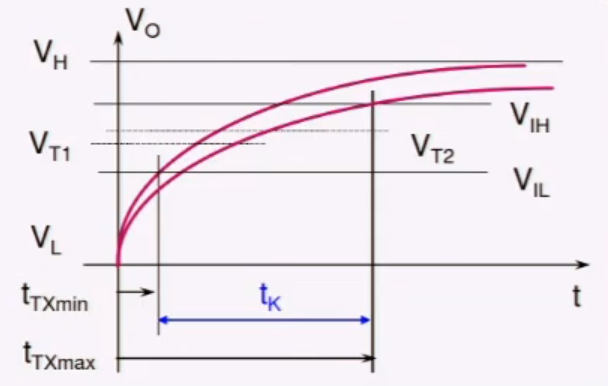
\includegraphics[width=0.5\textwidth]{variazione_di_ttx.png}
    \caption{Variazione Di Skew}
    \label{fig:variazione_di_skew}
\end{figure}


\section{Modelli a Linea}
Si studia la propagazione di segnali all'interno di un filo, dove gli obbiettivi sono:
\begin{itemize}
    \item massima velocit\`a;
    \item assenza di errori;
\end{itemize}

Modello RC: il filo presenta un resistenza in serie ed una capcit\`a a massa che rappresenta le capcit\`a parassite.

Si pu\`o considerare un filo composto da piccoli pezzettini, dove le resistenze in serie e parallelo possono essere trascurate, portando questi pezzettini a lunghezza infinitesima si ottiene la \textbf{linea di trasmissione}. Se le resistenze sono trascurabili la linea \`e detta \textbf{senza perdite} (induttanze e capicit\`a non dissipano potenza).

\subsection{Paramentri di una Linea di Trasmissione}
I parametri sono:
\begin{itemize}
    \item $Z_{\infty}$: impedenza caratteristica;
    \item lunghezza;
    \item velocit\`a di propagazione;
    \item tempo di propagazione;
\end{itemize}

Se la linea \`e senza perdita il segnale in entrata passa in modo intatto all'altra parte della linea.

\textbf{Trasmissione senza perdite}:
\begin{itemize}
    \item R in serie nulle: buon conduttore;
    \item G parallelo nullo: buon isolante;
\end{itemize}

\textbf{Con perdite}:
\begin{itemize}
    \item all'interno di circuiti integrati;
\end{itemize}

Si pu\`o definire la capacit\`a e l'induttanza per metro di linea:
\begin{itemize}
    \item $L_u$: induttanza unitaria;
    \item $C_u$: capcit\`a unitaria;
\end{itemize}

Il \textbf{parametri elettrici}:
\begin{itemize}
    \item impedenza caratteristica:
        \[ Z _{\infty} = \sqrt{\frac{L_u}{C_u} } \]
    \item velocit\`a di propagazione:
        \[ P = \frac{1}{\sqrt{L_uC_u}}  \]
    \item tempo di propagazione (tempo che impiega il segnale per spostarsi lungo la linea):
        \[ t_P = \frac{L}{P}  \]
\end{itemize}

Sono costretto ad usare un modello a linea quando i tempi di transizione ($t_r, t_f$) sono piccoli rispetto ai tempi di propazione ($t_P$).


\subsection{Riflessioni}
Supponiamo di avere un driver collegato al nodo B, che entra in una linea di trasmissione con: $Z _{\infty}$ e $t_P$. All'ingresso avr\`o un segnale attenuato, dato dal partitore tra $R_O$ e $Z _{\infty}$.
\begin{figure}[H]
    \centering
    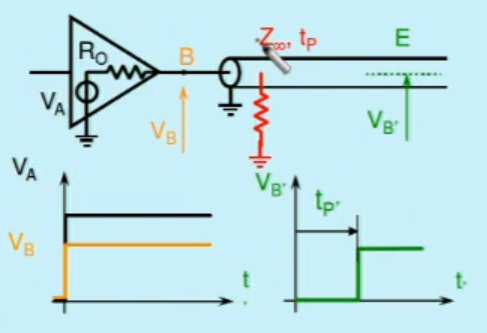
\includegraphics[width=0.5\textwidth]{liea-pilotata-con-gradino.png}
    \caption{Liea Pilotata Con Gradino}
    \label{fig:liea-pilotata-con-gradino}
\end{figure}

Il gradino che si sposta progressivamente dal trasmettitore a ricevitore \`e detta \textbf{onda progressiva}, dove in ogni punto della linea vale $Z _{\infty} = \frac{V(t)}{I(t)} $, che rimane costante. Se si ha una variazione di impedenza in un punto della linea (passaggio da una $Z _{\infty1}$ a $Z _{\infty2}$), il circuito non \`e dissipativo, dunque il rapporto $\frac{V}{I}$ deve variare, questo porta la nuova $Z _{\infty}$ a non assorbe tutta l'energia dell'onda progressiva, quindi l'unica soluzione \`e che la linea genera un'onda che ritorna indietro, l'onda che torna indietro \`e detta \textbf{onda riflessa}. Il segnale riflesso viene riflesso a sua volta quando torna indietro e cos\`i via, creando una serie di rimbalzi infiniti.

L'onda riflessa ha ampiezza:
\[ \boxed{V_r = \Gamma_T V_p} \]
Con $V_r$: tensione riflessa; $V_p$: tensione propagata.
\begin{definition}{Coefficente di Riflessione}{coefficente-di-riflessione}
    \[ \Gamma_T = \frac{R_T - Z_{\infty}}{R_T + Z _{\infty}}  \]
\end{definition}

In generale l'onda riflessa ha un'ampiezza, dopo una discontinuit\`a da $Z _{\infty}$ a $Z_1$ di:
\[ V_r = \Gamma_1 V_p \implies \Gamma_1 = (Z_1 - Z_{\infty})/(Z_1+Z _{\infty}) \]

Nel caso dinamico si aggiunge una \textbf{terminazione} che ha impedenza infinita pi\u` vicino possible alla $Z _{\infty}$ della linea, collegata al terminale del receiver.

Per rappresentare le trasmissioni si usa (la pi\`u comune) un diagramma a traliccio.
\begin{figure}[H]
    \centering
    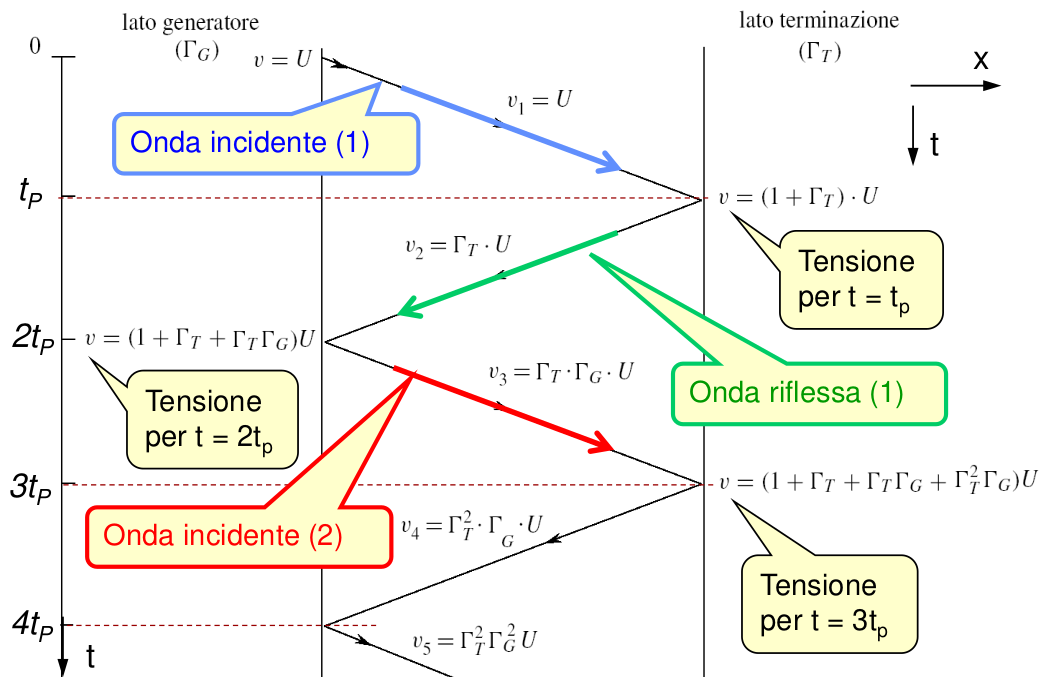
\includegraphics[width=0.8\textwidth]{diagramma-a-traliccio-della-riflessione.png}
    \caption{Diagramma A Traliccio Della Riflessione}
    \label{fig:diagramma-a-traliccio-della-riflessione}
\end{figure}

Ogni coefficente \`e minore di 1 (la successione converge a 0), questo porta le riflessioni a convergere verso un valore.


\section{Connessione con Linee}
It tempo di skew \`e dato dal tempo di trasmissione massimo meno il minimo.\\
Parametri del trasmettitore e ricevitore: $V_{OH|OL|IH|IL}$.
I parametri che influenzano $t _{TX}$ e $t_K$:
\begin{itemize}
    \item parametri di TX e RX ($V_H, V_L$ e $V_T$);
    \item propagazione: riflessioni, terminazioni (impedenze all'inizio ed alla fine), disconuit\`a, diafonia;
    \item carico (in particolare cariche capacitivi);
    \item rumore di massa;
\end{itemize}

\subsection{Tipologie di Connessione}
Collegamenti punto-punto: un unico driver e receiver, dove le condizini di propagazinoe sono ben definite.

Collegamenti a BUS: si possono collegare pi\`u periferiche diverse tra di loro, c'\`e uno o pi\`u driver, anche nel mezzo della linea, che comunicano con pi\`u receriver diversi tra di loro.

La struttura di riferimento sar\`a:
\begin{figure}[H]
    \centering
    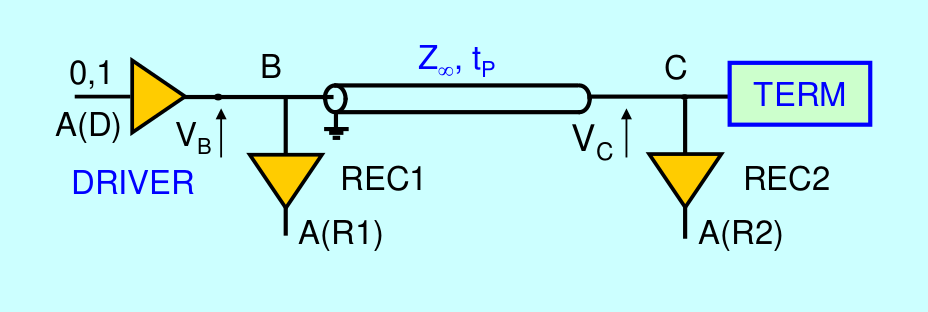
\includegraphics[width=0.6\textwidth]{struttura-di-riferimento-punto-punto.png}
    \caption{Struttura Di Riferimento Punto Punto}
    \label{fig:struttura-di-riferimento-punto-punto}
\end{figure}
Il primo gradino viene impresso dal driver, che viene caricato da $Z _{\infty}$, la terminazione determina una riflessione. Suppuniamo:
\begin{itemize}
    \item basso $R_O/Z _{\infty} \to$ bus veloci: l'onda incidente \`e molto ampia e non sono necessiare riflessioni, ma il coefficente sul driver \`e minore di 1, dunque potrebbero crearsi delle oscillazioni e dunque provocare delle commutazioni multiple nel receiver. Ci vuole un driver ad alta corrente, la terminazione dissipa energia.
    \item alto $R_O/Z _{\infty} \to$ bus lenti (possono volerci pi\`u riflessioni per superare la tensione di soglia): il primo gradino \`e basso, dunque si hanno bisogno di pi\`u riflessioni per raggiunger la soglia, ma avendo $R_O$ alto il coefficente al driver \`e positivo dunque non si creano oscillazioni. I due coefficenti di riflessione sono positivi, il motivo per cui anche il $\Gamma_R$ \`e positivo, implica che la resistenza al receiver \`e maggiore di quella del driver, se non fosse cos\`i la resistenza sarebbe vicino a massa, e le riflessioni tenderebbero asintoticamente a $0V$. Con driver a bassa corrente la tensione di soglia viene attraversata dopo diversi tempi di propagazione. Se l'andamento \`e molto lento il tempo di skew diventa molto alto (la differenza tra i tempi trasmissione massimo e minimo sono molto alti).
    \item driver adattato $R_O = Z _{\infty}$: adattamento lato driver, il primo gradino \`e pari alla met\`a della tensione a vuoto, si deve aspettare almeno una riflessione per superare la tensione di soglia. L'onda riflessa non si riflette a sua volta, il motivo \`e che il coefficente al driver \`e nullo ($R_O = Z _{\infty}$). Ha anche un consumo minore perch\`e non c'\`e bisogno di adattamento al receiver (\emph{far end}).
\end{itemize}

\subsection{Tipi di Terminazione}
\textbf{Terminaione in Parallelo}: terminazione tra il filo della linea e massa (o una tensione fissa, come la tensione di alimentazione). Se metto una $R_T = Z _{\infty}$ non ho riflessione. Ha basso ritardo ed alti consimi ma pu\`o essere pilotato in un punto intermedio.

\textbf{Terminaione in Serie}: adatto il driver con una $R_S$ tale che: $R_S + R_O = Z _{\infty}$. Ho anche una $\Gamma_T = 1$. Ha basso velocit\`a e bassi consumi ma non pu\`o essere pilotato in punto intermedio.

Gli effetti del carico capacitivo diminuiscono l'impedenza caratteristice e la velocit\`a di propagazione. Questo rendi il sitema pi\`u lento e rende il driver non pi\`u adattato, oltre ad aumentare la potenza consumata. Bisogna limitare gli effetti delle cariche capacitive, ad esempio un clock che deve far commutare 100 driver, si usa un buffer che carica i drivver al posto della linea diretta.

\subsection{Collegamenti Multi-Punto}
Nei BUS si devono cercare di limitare le derivazioni ed i carichi capacitivi (se colleghiamo il BUS direttamente la capacit\`a totale vista all'inizio della linea sar\`a molto ampia, dunque i tempi saranno lunghissimi, ad avare tutte i carichi capacitivi dati dai driver e dai receiver presenti sulla linea), per evitre questo non si collega mai un linea in modo diretto alla piastra ma si usano, ad esempio, dei \textbf{transceiver} o dei buffer.

Vediamo come l'effetto dei tensioni viene passata al livello superiore nella gerarchia ISO/OSI. Per ottenere velocit\`a elevate occorre minimizzare lo skew e garantire delle specifiche temporali, creando cos\`i dei protocolli a livello di ciclo, che devono garantire l'integrit\`a dei dati trasmessi.


\subsection{Problemi}

\begin{problem}{}{}
    Un'interconnessione punto-punto ha:
    \begin{itemize}
        \item $Z_{\infty} = 70\Omega; t_p = 10ns$;
        \item Receiver: $V_{AL} = 5V; V _{IH} = 3V; V _{IL} = 0.8V$;
    \end{itemize}
    Calcolare i coefficenti di riflessione al driver ed al receiver, il tempo di trasmissione e skew per le coppie di resitenze:
    \[ (R_O,R_T) \implies (100, \infty); (100, 200); (50, 200); (50, 100); (10, 100); (10, 10); \]
    \begin{itemize}
        \item $(100, \infty)$:
            \[ \Gamma_D = 0.18 ;\; \Gamma_R = 1 \]
            \[ t_{TX} =  ;\; t_K =   \]
        \item $(100, 200)$:
            \[ \Gamma_D = 0.18 ;\; \Gamma_R = 0.48 \]
            \[ t_{TX} =  ;\; t_K =   \]
        \item $(50, 200)$:
            \[ \Gamma_D = -0.16 ;\; \Gamma_R = 0.48  \]
            \[ t_{TX} =  ;\; t_K =   \]
        \item $(50, 100)$:
            \[ \Gamma_D =  -0.16 ;\; \Gamma_R =  0.18 \]
            \[ t_{TX} =  ;\; t_K =   \]
        \item $(10, 100)$:
            \[ \Gamma_D = -0.75 ;\; \Gamma_R = 0.18 \]
            \[ t_{TX} =  ;\; t_K =   \]
        \item $(10, 10)$:
            \[ \Gamma_D =  -0.75 ;\; \Gamma_R = -0.75 \]
            \[ t_{TX} =  ;\; t_K =   \]
    \end{itemize}
\end{problem}

\newpage
\section{Cicli Base di Trasferimento}
Esistono due metodi per creare una sincronizzazione tra la linee di trasmissione: sincrona (scandita da un clock), asincrona. Si passa dal livello \textbf{fisico} al livello \textbf{cilco}. Nel livello di ciclo si trasferiscono singoli stati logici: interpretati a partire da delle tenioni. Nel livello di ciclo si trasferiscono gruppi di bit: i vincoli importanti da rispettare sono i tempi di set-up e di hold, visto che si opera con dei FF.

Per trasmettere un dato si necessitano di almeno due segnali (uno porta il dato, uno porta il clock ad esempio). Al driver ed al receiver si devono ripettare i tempi di setup e di hold. Date due linee di trasmissione esistono due tempi $t_1$ e $t_2$ ($t_0 =$ tempo iniziale):
\[ t_1 = t_0 + t _{TXmedio} + t_K \]
\[ t_2 = t_0 + t_{su(D)} + t_{TXmedio} \]
La differenza tra questi due tempi \`e proprio il tempo di setup del receiver:
\[ t _{su(R)} = t_2 - t_1 = t _{su(D)} - t_K \]
Lo skew riduce i margini di temporizzazione.

 \subsection{Sorgente-Destinazione}
Per modellare questi ritardi si una modello \textbf{sorgente-distinazione}, la destinazione \`e un FF che fa una fotografia in un istante in cui si \`e sicuri che tutti i bit abbiano un giusto valore. Il clock comune a tutti i FF non viene collegato direttamente ma viene usato un buffer, che ha il vantaggio di avere riflessioni molto pi\`u lente che non con un collegamento diretto al clock. 

Esistono due tipi di trasmissione di dati:
\begin{itemize}
    \item Una sorgente vuole \textbf{srivere} dei dati su un destinatario: la sorgente manda i dati ed segnale di controllo verso una destinazione;
    \item Una destinazione vuole \textbf{leggere} dei dati da una sorgente: la destinazione \\ richiede dei dati, il flusso dei dati e dei segnali di controllo viaggiano in verso opposto;
\end{itemize}
Per evitare la metastabilit\`a i tempi di setup e hold devono essere rispettati, due tecniche base sono: protocollo sincrono (a temporizzazione fissa, dove vengono dati dei riferimenti temporali fissi, dove vengono cosiderati sempre i casi peggiori, solitamnte scanditi da un clock); temporizzazione asincrono (temporizzazione adattiva, dove i tempi sono variabili e le terminazioni delle operazoini sono dettate da dei segnali di ACK).

\subsection{Scrittura}
Si hanno cicli di scrittura con dei ritardi fissi ($t_A, t_B$), dove c'\`e un intervallo temporale di scambio di informazioni, al termine di questo inervallo i dati non cambiano pi\`u. Essendoci dei ritardi prefissati noti a priori \`e possibile rispettari i vincoli sul ricevitore di setup e di hold, perch\`e tutti i parametri sono controllati dalla sorgente.

Al tempo $t_0$ i dati sono stabili, al ricevitore i dati sono incerti prima dell'arrivo dei dati dal ricevitore, dunque il tempo dopo la quale i dati al ricevitore saranno stabili sar\`a il tempo di ritardo massimo, perch\`e come al solito si devono considerare i casi peggiori, ma anche il datsar\`a anche stabile per meno tempo, perch\`e il tempo minino dopo che i dati non vengo pi\`u trasferiti dal trasmettitore \`e il tempo minimo di trasmissione. Il tempo di setup \`e il tempo in cui l'input deve essere grantito stabile prima del colpo di clock al FF, questo tempo corrisponde alla differenza tra l'ultima transizione del dato alla prima transizione del clock: $t_{su} = t_A + t_{TXmin} - t_{TXmax} = t_A - t_K > t_{su(FF)}$.

Analogamnte per il tempo di hold, si calcola: $t_h = t_B + t_{TXmin} - t_{TXmaz} = t_B - t_K > t_{h(FF)}$, dove la scelta dei tempi dipende solo dallo sckew e dei tempi di setup. Anche qui lo sckew diminuisce i margini di temporizzazione. Con questo metodo si possono calcolare i valori di $t_A$ e $t_B$, in modo da rispettare i vincoli sul destinatario.

Nei casi di scritture \textbf{broadcast} (scritture sui pi\`u destinatari contemporaneamente), si devono rispettari i tempi del destinatario pi\`u lento.

\subsection{Ciclo Asincrono}
Di base si ha sempre una sergente che trasmette dei dati ad una destinazione, come prima si ha una transizione per strobe. Lo strobe arriva ad una macchina a stati che determina quando mandare il tempo di clock al FF ed inoltre manda indietro al trasmettitore un segnale di ACK. L'interlacciamnento STB/ACK \`e detta \textbf{handshake}.
\begin{figure}[H]
    \centering
    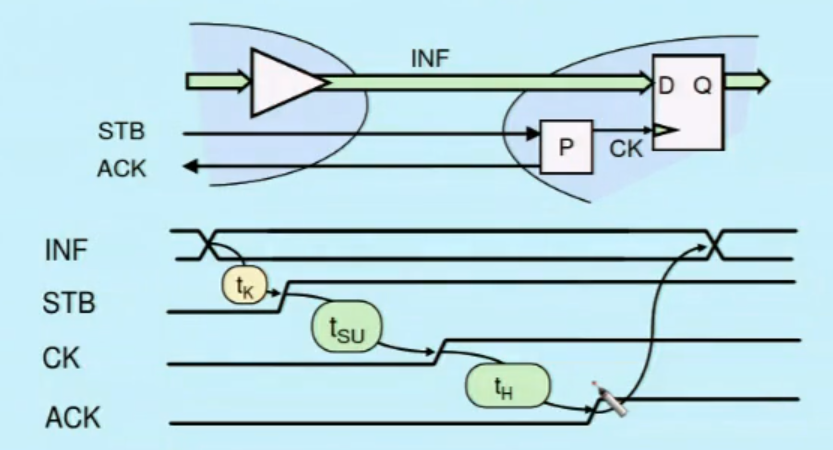
\includegraphics[width=0.5\textwidth]{ciclo-asincrono.png}
    \caption{Ciclo Asincrono}
    \label{fig:ciclo-asincrono}
\end{figure}
I ritardi (di setup, di hold e di skew) generati dalla macchina a stati, sono creati da un ulteriore clock ad alta frequenza che attraverso un logica sincrona che conta il ritardo, \`e molto conveniente usare un clock a frequenza pi\`u alta perch\`e la logica ascincrona \`e molto lenta duqnue, \`e molto facile generare un clock con dei margini elevati.

Quando l'ACK al trasmettitore deve essere a 0 prima di far ripartire un ciclo sono detti \textbf{cicli chiusi}, altrimenti \textbf{cicli aperti} in cui l'analisi \`e pi\`u complicata ma sono pi\`u efficenti.


\newpage
\section{Protocolli di BUS}
Le tecniche di indirizzamento sono gestite da un singolo master, i sistemi con pi\`u master 
I servizi forniti dal livello di ciclo forniscono dei dati fornendo delle specifiche temporali. Il livello di ciclo non si interessa del tipo di dato trasmesso. I protocolli estesi permettono il trasferimento di dati in madalit\`a 1-a-N e N-a-M (N master e M master). Fornire questi servizi comporta un consumo di energia e di tempo, determinari dal livello di ciclo.

Vengono definiti degli indirizzi per identificare i diversi dati, uno o pi\`u dati posso essere passati da un sistema ad un altro, questo viene detto \textbf{transazione}, dove si passa un unico pezzo di informazione, il master incomincia la transazione.

Il trasferimento punto-punto comporta la conoscenza completa del trasmettitore e del ricevitori.

I sistemi multi-punto comprendono pi\`u master e pi\`u slave. Pi\`u unita usano lo stesso BUS fisico, una volta identificati i participanti alla transazione si iniziono i cicli di lettura o scrittura.

Nei sistemi a BUS \`e possible rimuovere o aggiungere dei moduli (\textbf{sistema modulare aperto}), avento tempi di sckew, setup e hold variabili (non sono uguali per moduli diversi). Non \`e possibile mettere un numero indefinito di moduli perch\`e comporterebbe ad un ritardo massimo indeifinto, per questo motivo si definiscono delle regole ben procise a cui tutti i moduli devono obbedire (protocolli), altrimenti si rompe tutto.

Se devo collegare pi\`u sistemi in modalit\`a punto-punto le specifiche sono ben definite, questo per\`o richiede di fare delle procedure di routing, mentre nel mutlipunto ho un unica BUS dove l'unica azione che deve essere performata \`e l'arbitraggio. Nel punto-punto si ottengono velocit\`a maggiori che nul multi-punto, nul multi-punto si deve tenere conto del sistema pi\`u lento, oltre a mantenere un'informazione che rappresenta il destinatario.

Nei sistemi a BUS si devono considerare dei cicli specifici per selezionare le unit\`a partecipanti, in particolare decidere il master e lo slave. Genericamente c'\`e prima una fase di allocazione(l'unico master che pu\`o utilizzare il canale), l'indirizzamente (la decisione dello slave), il trasferimento dei dati tra master e slave.

\textbf{Sistemi a singolo master}: nello slave c'\`e un qualcosa che decodifica l'indirizzo comunicato dallo slave, che permette di decidere quale slave il master inizia a comunicare, per fare ci\`o si usano dei comparatori, decodificatori e logica. Ci sono delle temporizzazzioni che dopo il riconoscimento della connessione col master partono i controlli per lo strobe, e gli altri segnali. Questi dati si trovano all'interno dello slave allocati in una parte specifica del circuito, che verranno gestiti attraverso degli indirizzi, per distinguerli tra di loro. Per velocizzare la trasmissione si utilizzano anche negli slave dei buffer verso il BUS.

\subsection{Tecniche di Indirizzamento}
Per indirizzare gli slave esistono due tipi di selezione:
\begin{itemize}
    \item codificata: ho N bit che selezionano 1 elemento tra $2^{N}$ elementi, ogni elemento ha un indirizzo assegnato a lui codificato;
    \item decodificata: si quando si hanno pochi slave collegati al BUS, la selezione avviene su M bit tra M diversi slave;
\end{itemize}
La selezione decodificata a differenza di quella codificata \`e pi\`u veloce perch\`e non va effettuata la decodifica.

L'indirizzamento pu\`o essere geografico (dove la selezione dipende dalla posizione rispetto agli slot collegati al BUS), o logico (dove la selezione dello slave dipende dal suo nome).

\subsection{Protocolli Multi-Punto}
Occorre identificare la coppia master-slave, che pu\`o essere decisa da un'unit\`a centrale o dalla decisione comune. Quando due master richiedono contemporaneamente l'utilizzo del BUS viene generata una \textbf{collisione}, che assolutamnte evitata.

Un meccanismo per prevenire la collisione \`e un meccanismo a \textbf{token}: il gettone viene passato da master a master, nel momento in cui uno di loro deve usare il BUS ed ha il gettone in mano lo blocca per se ed inizia ad utilizzarlo, se non ha nessuna richiesta da fare lo passa al prossima master, per relizzare questo si devono definire dei meccanismi per passare il token.

Un altro meccanimso \`e quello del \textbf{collision detection}: se un master si accorge che il BUS \`e gia in uso, stoppa la sua connessione ed aspetta un tempo casuale prima di riconnettersi, altrimeti lo utilizza.

Un altro meccanimso \`e l'\textbf{arbitraggio}: un'unit\`a centrale gestisce le rechieste e valuta a chi dare l'autorizzazione per il BUS, per gestire l'arbitraggio esistono due politoche:
\begin{itemize}
    \item \textbf{temporale}: si usa politica first come first served;
    \item \textbf{logica}: si definisce una priorit\`a diversa per le differenti periferiche, dove alcune hanno il diritto di precedenza sulla altre, utilizzando questa politica si deve evitare la \textbf{starvation};
\end{itemize}



\subsection{Valutazione di Prestazioni}
Le prestazioni si misurano attraverso dei paramettri, il pi\`u importante \`e il \textbf{throughput}, che \`e uguale al numero di bit trasferiti nell'unit\`a di tempo:
\[ T = \text{larghezza del bus} \times \text{velocit\`a del bus} \]
La velocit\`a del BUS si mirura in cilci al secondo: $ = \frac{1}{t_c} $. La durata del ciclo $t_x$ dipende da: parametri elettrici, parametri del modulo e dai parametri del protocollo.

Anche qui si hanno dei protocolli per il trasferimento dei dati, che possono essere sincroni ed asincroni. Il protocollo migliore \`e il \textbf{source synchronous} che permette ad entrambe le untit\`a che stanno comunicando di gestire i segnali di controllo, in questo modo \`e necessario conoscere solo i ritardi.

I \textbf{BUS multiplati} sono le strutture base per BUS paralleli: infatti sui BUS multiplati gli indirizzi, i dati e i segnali di controllo viaggiano sulgi stessi conduttori, il motivo \`e che \`e molto oneroso in termini di spazion e di costo aver molti conduttori, pin, driver e receiverdiversi per ogni tipo diverso di dato. C'\`e bisogno di scandire dei cicli in cui ogni viaggiano solo dei tipi di dato nello stesso istante.

Un alro modo di migliorare le prestazione \`e nel ciclo standar di lettura e scrittura ci sono due cicli. Il consumo \`e dato dal numero di transazioni che vengono effettuate, durante una transazione si hanno due transizioni (una verso l'alto ed una verso il basso), viene sfruttato allora un cilce di \textbf{Double Data Rate} (\textbf{DDR} o \textbf{Dual-edge}), che sfrutta entrambe le transizioni dei segnali, compresi lo strobe e l'ACK, migliorando in questo modo i consumi e la velocit\`a.

Source cynchronous

La parte di trasferimento del dato, di solito, \`e solo una piccola frazione del tempo di ciclo, nel trasferimento a blocco si fa un solo arbitraggio, mendando un unico indirizzo si iniziano a mandare quelli successivi, fino a N blocchi. Questo viene fatto perch\`e \`e molto probabile che i dati necessari siano vicini all'indirizzo che si \`e richiesto. Nelle memorie a indirizzamento a blocchi c'\`e bisongo di una logica di controllo prima della memoria che ricevuto un indirizzo genera quelli successivi che andranno a prendere i dati in memoria.

\subsection{Domande}
Quando e perché deve essere presente una operazione di indirizzamento?
In quali sistemi è necessaria una operazione di arbitrazione?
Descrivere il funzionamento di un arbitro di bus.
Cosa si intende per “prestazioni” di un bus?
Indicare i parametri che determinano le prestazioni di un bus.
Da cosa dipende il tempo di ciclo minimo?
Confrontare i tempi minimi di ciclo per protocolli sincroni e asincroni.
Descrivere i vantaggi dei protocolli DDR.
Quali vantaggi si ottengono con i bus multiplati?
Descrivere i vantaggi di transazioni con trasferimento a blocchi.


--- Se ci sono pi\`u slave, o se ho una memoria con molti dati;

--- Quando si hanno pi\`u master;

--- Decide chi \`e il master attraverso dei meccanismi di: token passing, collision detection, priority queue o coda LIFO;

--- Dipende dal throughput (bit o byte o parole al secondo);

--- Dimensione e tempo di ciclo (tempo di trasferimento, sckew, tipo di protocollo, se sincrono o asincrono, dual data rate, suorce synchronous);

--- Che vengono sfruttate entrambe le transizioni del clock (velocit\`a doppia e consumi ridotti);

--- Meno connessioni, meno trasizioni, meno consumo, meno materiale, pi\`u logica per gestire i tipi diversi di dati.

---  Meno tempo di indirizzamento, trasmettere pi\`u dati con un solo indirizzamento;





\newpage
\section{Collegamenti Seriali}
 Nella connessione seriale si ha un unico filo che trasmetti i dati in tempi successivi. Nel trasferimento vengono usati degli shift register per convertire i dati da parallelo a seriale e viceversa. Il trasferimento di N dati comporta N cicli. I pochi segnali riducono le interferenza elettromagntiche e il disallineamento temporale, causato dallo skew.

 Esisteno dei collegamenti autosincronizzanti dove il clock viaggia sullo stesso filo dei dati (detto \textbf{clock-data embedding}). Il vantaggio dei collegamenti seriali \`e il ridotto numero di conduttori, alte velocit\`a su lunghe distanze.  I problemi del trasferimento serialo sono il trasferimento di N simboli diversi, oltre ad avere dei proble di sincronizzazione con il sistema ricevente.

 Si parla di bit-rate per rappresentare il numero di bit al scecondo, ed di buad-rate, ovvero di numero di simboli al secondo. Esistono simboli binari, come l'NRZ: Non Return to Zero, e l'RZ: Return to Zero.

 L'interferenza intersimbolica \`e l'interfernza causata da fili che si trovano vicini alla linea di trasmissione, che compartano un aumento del tempo di ciclo, il motivo \`e che porta e del rumore. Nel collegamento in parallelo viene detto \textbf{diafonia}, mentre nei seriali \`e detto \textbf{Inter Symbolic Interference}, causato dalle riflessioni sul filo, anche sul bit successivo. 

 I collegamenti sono fatti da passaggi da un registro PISO ad uno SIPO, i dati vengono trasferiti su una linea di trasferimento.


















\newpage
\section{Cicli di Trasferimento}
Come abbiamo gi\`a visto lo scopo delle linee di collegamento \`e qeullo di trasferire i dati tra pi\`u sistemi. Si deve passare necessariamente dal livello \textbf{fisico}, il trasferimento dei singoli bit, che introduce del rumore. Per trasferire dei dati \`e necessario definire dei protocolli per interpretare i dati.

A livello di \textbf{ciclo}, ovvero al livello di trasferimento di gruppi di bit (e.g. byte), il protocolle deve assicurarsi che all'arrivo del gruppo di bit, essi siano corretti ed abbiano un ritardo ben definito. Per descrivere un sistema i bit che viaggiano in parallelo hanno dei vincoli diversi, dati dai diversi parametri che ogni linea possiede. Appena si ha la certezza che i dati sono arrivati con certezza di procede a passare i dati al sistema.

Questi sistemi fanno affidamento su un livello fisico che viene gestito da un driver che passa i dati attraverso un collegamento che arrivano ad un reciver, che decofica i dati che gli arrivano e poi converti i segnali in dati per il sistema a cui \`e collegato.




\newpage
\section{Integrit\`a di Segnale}
La diafonia \`e un aspetto di interazione tra pi\`u linee, in cui il segnale su ogni linea interferisce direttametne con i segnali scambiati sulle altre linee.

Il \textbf{Crosstalk} o la \textbf{diafonia} \`e il passaggio di seganle. Gli accoppiamenti che si vengono a creare sono di tipo: induttivo e capacitivo tra conduttori diversi o di accoppiamento per maglie comuni per lo stesso conduttore.

\subsection{Accoppiamento tra Conduttori}
Le linee vicene tra di loro, possono avere degli accoppiamenti induttivi o capacitivi, causate dai disturbi elettromagnetici.
\begin{figure}[H]
    \centering
    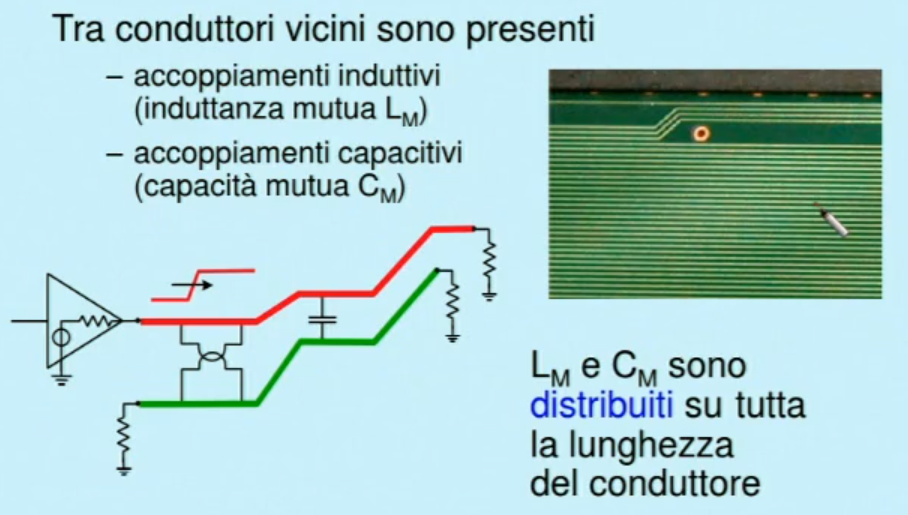
\includegraphics[width=0.5\textwidth]{accoppiamnto-tra-conduttori.png}
    \caption{Accoppiamnto Tra Conduttori}
    \label{fig:accoppiamnto-tra-conduttori}
\end{figure}

Qunando si ha un linea pilotata, essa crea un disturbo, detta \textbf{linea disturbante}. Qunado il driver invia un segnale ci sono delle riflessioni, supponendo che la \textbf{linea disturbata} abbia una terminazione adattate, sulla linea si vede un linea incidente ed un onda riflessa.

I parametri di accoppiamento sono, e vengono causati dalla uniche transizioni dei segnali, i disturbi sono legati alla pendenza dei fronti. 

Per ridurre il crosstalk si possono rallentare i fronti di salita (comporando un rallentamento dell'intero sistema) oppure usando dei segnali diffenziali (ognuno compensa gli errori dell'altro). Oppure si possono ridurre gli effeti del crosstalk mettendo: un filtro nel receiver o usando della tecniche di ritrasmissione dei dati.

\subsection{Riduzione la Pendenza dei Fronti}
Per ridurre la pendenza (derivata, $\frac{dv}{dt} = \frac{\Delta V}{\Delta t}$). Si pu\`o ridurre $\Delta V$, con un consumo minore di potenza) o aumentare $\Delta t$ con un uso di logica pi\`u lenta.

\subsection{Accoppiamenti Induttivi}
...

I vantaggi dei segnali differenziali, hanno immunit\`a al segnale di \textbf{modo comune}, di pu\`o ridurre l'escursione senza senza l'aumento della sensibilit\`a al rumore, inoltre la corrente totale \`e costante.

Gli svantaggi sono che si devono usare due piste e 2 piedini per ciascun segnale, inoltre richiede delle tecniche analogiche per ricostruire il segnale.

La distribuzione del clock comporta dei disturbi. O

...




\section{Sistemi di Conversione A/D/A}
I segnali analogici (continui nel tempo e nell'ampiezza), sono campionati in segnali digitali. Si hanno due discretizzazioni 












\newpage
\section{Esercizi}

\subsection{Porte Logiche CMOS}

\begin{problem}{}{}
    \begin{enumerate}
        \item Completare lo schema logico in figura;
        \item Calcorare la $t_{rise}$ al nodo E;
        \item Calcolare la $t_p$ della rete di pull-up e dell'inverter sapendo che all'uscita sono collegati 10 inverter;
    \end{enumerate}
    I MOS hanno le seguenti caratteristiche:
    \[ R _{on} 10k\Omega;\quad C _{gate} = 5fF;\quad V _{dd} = 1.5V .\]
    % TODO:  <16-03-22, mettere foto> %
    
    \emph{Solution:}
    \begin{enumerate}
        \item Sium
        \item Fare traise
        \item $\to$
    \end{enumerate}
\end{problem}

\begin{problem}{}{}
    \begin{enumerate}
        \item Implementare una una porta cMOS con funzione: $U = (A\cdot B + C\cdot D)*$
        \item Determinare $t_p$ min e max sapendo che: $R _{on} = 20k\Omega$ e l'uscita $U$ \`e collegata ad un carico di $C=50fF$.
    \end{enumerate}
    
    \emph{Solution:}
    \begin{enumerate}
        \item  ok
        \item $ \implies $
            \[ \begin{system} 
                t _{pHL,min} = 0.69\cdot 50pF\cdot 20k\Omega = 0.69ns \\
                t _{pHL,max} = 0.69\cdot 50pF\cdot 40k\Omega = 1.4ns
            \end{system}  .\]
            \[ \begin{system} 
                t _{pLH,min} = 0.69\cdot 50pF\cdot 20k\Omega = 0.69ns \\
                t _{pLH,max} = 0.69\cdot 50pF\cdot 40k\Omega = 1.4ns
            \end{system}  .\]
    \end{enumerate}
\end{problem}

\begin{problem}{}{}
    
\end{problem}

\subsection{B2}
\begin{problem}{}{}
    \begin{figure}[H]
        \centering
        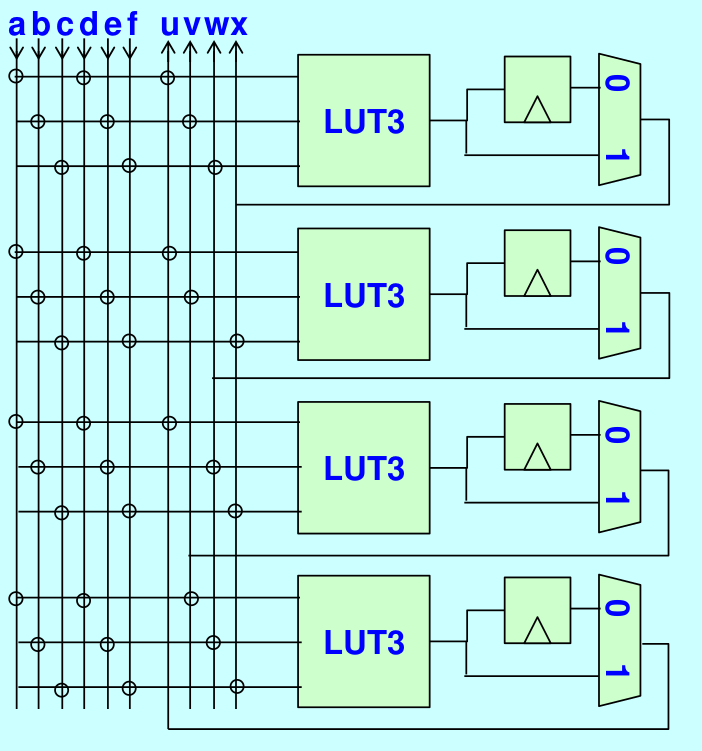
\includegraphics[width=0.8\textwidth]{logica-programmabile-1.png}
        \caption{logica-programmabile-1.png}
        \label{fig:logica-programmabile-1-png}
    \end{figure}
\end{problem}


\newpage
\section{Esami}

Il tempo di propagazione L-H di una porta CMOS NAND a 2 ingressi con una capacita di carico $C_G = 0.1fF$ collegata all'uscita $t_P = 200ps$. 


\end{document}
